\documentclass{beamer}
\usepackage[spanish, es-tabla]{babel} %Idioma

% Codificación
\usepackage[utf8]{inputenc}
\usepackage[T1]{fontenc}
\usepackage{qrcode}

% Paquetes matemáticos
\usepackage{amsmath, amssymb, physics, bigints, cancel}
\usepackage{stmaryrd}

% Colores y cuadros
\usepackage[most]{tcolorbox}
\usepackage[absolute,overlay]{textpos}
\setlength{\TPHorizModule}{1cm}
\setlength{\TPVertModule}{1cm}

\newtcolorbox{infobox}[2][blue]{
    colback=#1!5!white,
    colframe=#1!75!black,
    title={#2},
    fonttitle=\bfseries,
    coltitle=black,
    boxrule=0.8pt,
    arc=4pt,
    left=6pt,
    right=6pt,
    top=6pt,
    bottom=6pt,
    breakable
}

% TikZ para diagramas y circuitos
\usepackage{tikz}
\usetikzlibrary{patterns, decorations.pathreplacing}
\usepackage{circuitikz}

% Figuras
\usepackage{graphicx}
\usepackage{float} % no siempre necesario, pero puede ayudar

% Tablas pro
\usepackage{booktabs}

% Listados de código
\usepackage{listings}

% Bash personalizado
\lstdefinelanguage{custombash}{
    language=bash,
    morekeywords={conda, activate, mkdir, cd, cmake, make, git, sudo},
    sensitive=true
}

\lstdefinestyle{bashStyle}{
    language=custombash,
    basicstyle=\ttfamily\small,
    keywordstyle=\color{teal}\bfseries,
    commentstyle=\color{gray}\itshape,
    stringstyle=\color{orange},
    identifierstyle=\color{black},
    numbers=left,
    numberstyle=\tiny\color{gray},
    stepnumber=1,
    numbersep=10pt,
    backgroundcolor=\color{white},
    showspaces=false,
    showstringspaces=false,
    breaklines=true,
    frame=single,
    captionpos=b
}

% Python
\lstdefinestyle{pythonStyle}{
    language=Python,
    basicstyle=\ttfamily\small,
    keywordstyle=\color{blue}\bfseries,
    commentstyle=\color{gray}\itshape,
    stringstyle=\color{orange},
    identifierstyle=\color{black},
    numbers=left,
    numberstyle=\tiny\color{gray},
    stepnumber=1,
    numbersep=10pt,
    backgroundcolor=\color{white},
    showspaces=false,
    showstringspaces=false,
    breaklines=true,
    frame=single,
    captionpos=b
}

% C++
\lstdefinestyle{cppStyle}{
    language=C++,
    basicstyle=\ttfamily\small,
    keywordstyle=\color{blue}\bfseries,
    commentstyle=\color{gray}\itshape,
    stringstyle=\color{red},
    numbers=left,
    numberstyle=\tiny\color{gray},
    stepnumber=1,
    numbersep=10pt,
    backgroundcolor=\color{white},
    showspaces=false,
    showstringspaces=false,
    breaklines=true,
    frame=single,
    captionpos=b
}

% Fuente doble negrita
\usepackage{bbold}

% Íconos FontAwesome
\usepackage{fontawesome5}

% Para texto de ejemplo
\usepackage{lipsum}

% Comando para tachado en color
\newcommand{\colorcancel}[2]{\textcolor{#1}{\cancel{\textcolor{black}{#2}}}}

% Comando para círculos con texto
\newcommand*\circled[1]{\tikz[baseline=(char.base)]{
  \node[shape=circle,draw,inner sep=1.5pt] (char) {#1};}}

% Pie de página
\setbeamertemplate{footline}[frame number]

% Justificado
\usepackage{ragged2e} 
\usepackage{etoolbox}
\apptocmd{\itemize}{\justifying}{}{}
\apptocmd{\enumerate}{\justifying}{}{}

\usepackage{multicol,booktabs,calligra}
\usepackage{chancery}
\usepackage{contour}
\usepackage{subcaption}
\usepackage{xspace}
\usepackage{bm}
\contourlength{0.4pt}

% 1. Creamos el interruptor (por defecto está encendido)
\newif\ifmostrarindice
\mostrarindicetrue

% 2. Modificamos el comando para que respete el interruptor
\AtBeginSection[]
{
  \ifmostrarindice
    \begin{frame}
      \frametitle{Índice}
      \tableofcontents[currentsection, hideothersubsections]
    \end{frame}
  \fi
  \mostrarindicetrue % Importante: se vuelve a encender para la próxima sección
}

\newcommand{\CosmoLattice}{\ensuremath{\mathcal{C}}\text{osmo}\ensuremath{\mathcal{L}}\text{attice}\xspace}

\definecolor{ForestGreen}{rgb}{0.13, 0.55, 0.13}
\definecolor{esmerald}{RGB}{80, 200, 120}
\definecolor{gold}{RGB}{212, 175, 55}
\definecolor{silver}{RGB}{192, 192, 192}

\pagecolor{black}
\color{white}

\begin{document}
    \begin{frame}
        \begin{figure}[H]
            \centering
            \begin{tikzpicture}
                \node at (-0.5,0) {\bfseries \LARGE \color{black}\contour{gold}{\shortstack{Producción de ondas gravitacionales\\durante el Recalentamiento: análisis\\ teórico y simulaciones con\\\CosmoLattice}}};

                \node at (-0.5,-2.25) {\texttt{\color{black}\contour{silver}{Tomás Alejandro Ciccarella}}};

                \node at (-3, -4.5) {\texttt{\textbf{Director:} Nahuel Mirón Granese}};
                \node at (-3.175, -5) {\texttt{\textbf{Codirector:} Esteban Calzetta}};

                %\draw[fill = red, rounded corners = 2] (2.4,-4.35) rectangle ++(2.2,-0.7);
                %\draw[fill = white, rounded corners = 2] (2.5,-4.45) rectangle ++(2,-0.5);
                \node at (-5,-5.5) {\textrm{08/07/2026}};

                %\node at (-3.5,-5.5) {
\includegraphics[scale = 0.2]{Figures/logo_DF.png}};
                \node at (3,-4.5) {
\includegraphics[scale = 0.15]{Figures/logo_UBA.png}};
            \end{tikzpicture}
        \end{figure}
    \end{frame}

    \begin{frame}{\bf \textcolor{black}{Hoja de ruta}}
        \tableofcontents[hideallsubsections]
    \end{frame}

    \begin{frame}
        \begin{figure}[H]
            \begin{tikzpicture}
                \node at (0,0) {\Huge \color{black}\contour{gold}{\uppercase{Introducción}}};                
            \end{tikzpicture}
        \end{figure}
    \end{frame}

    \section{Introducción}

        \subsection{Cosmología}

            \begin{frame}{Historia del Universo}
                %\begin{center}
                %    \textrm{``Our whole Universe was in a hot dense state. Then nearly 14 billion years ago expansion started...''}
                    
                %    \textrm{``...And all started with a Big Bang''}
                %\end{center}
                \begin{figure}[H]
                    \centering
                    \begin{tikzpicture}
                        \node at (0,0) {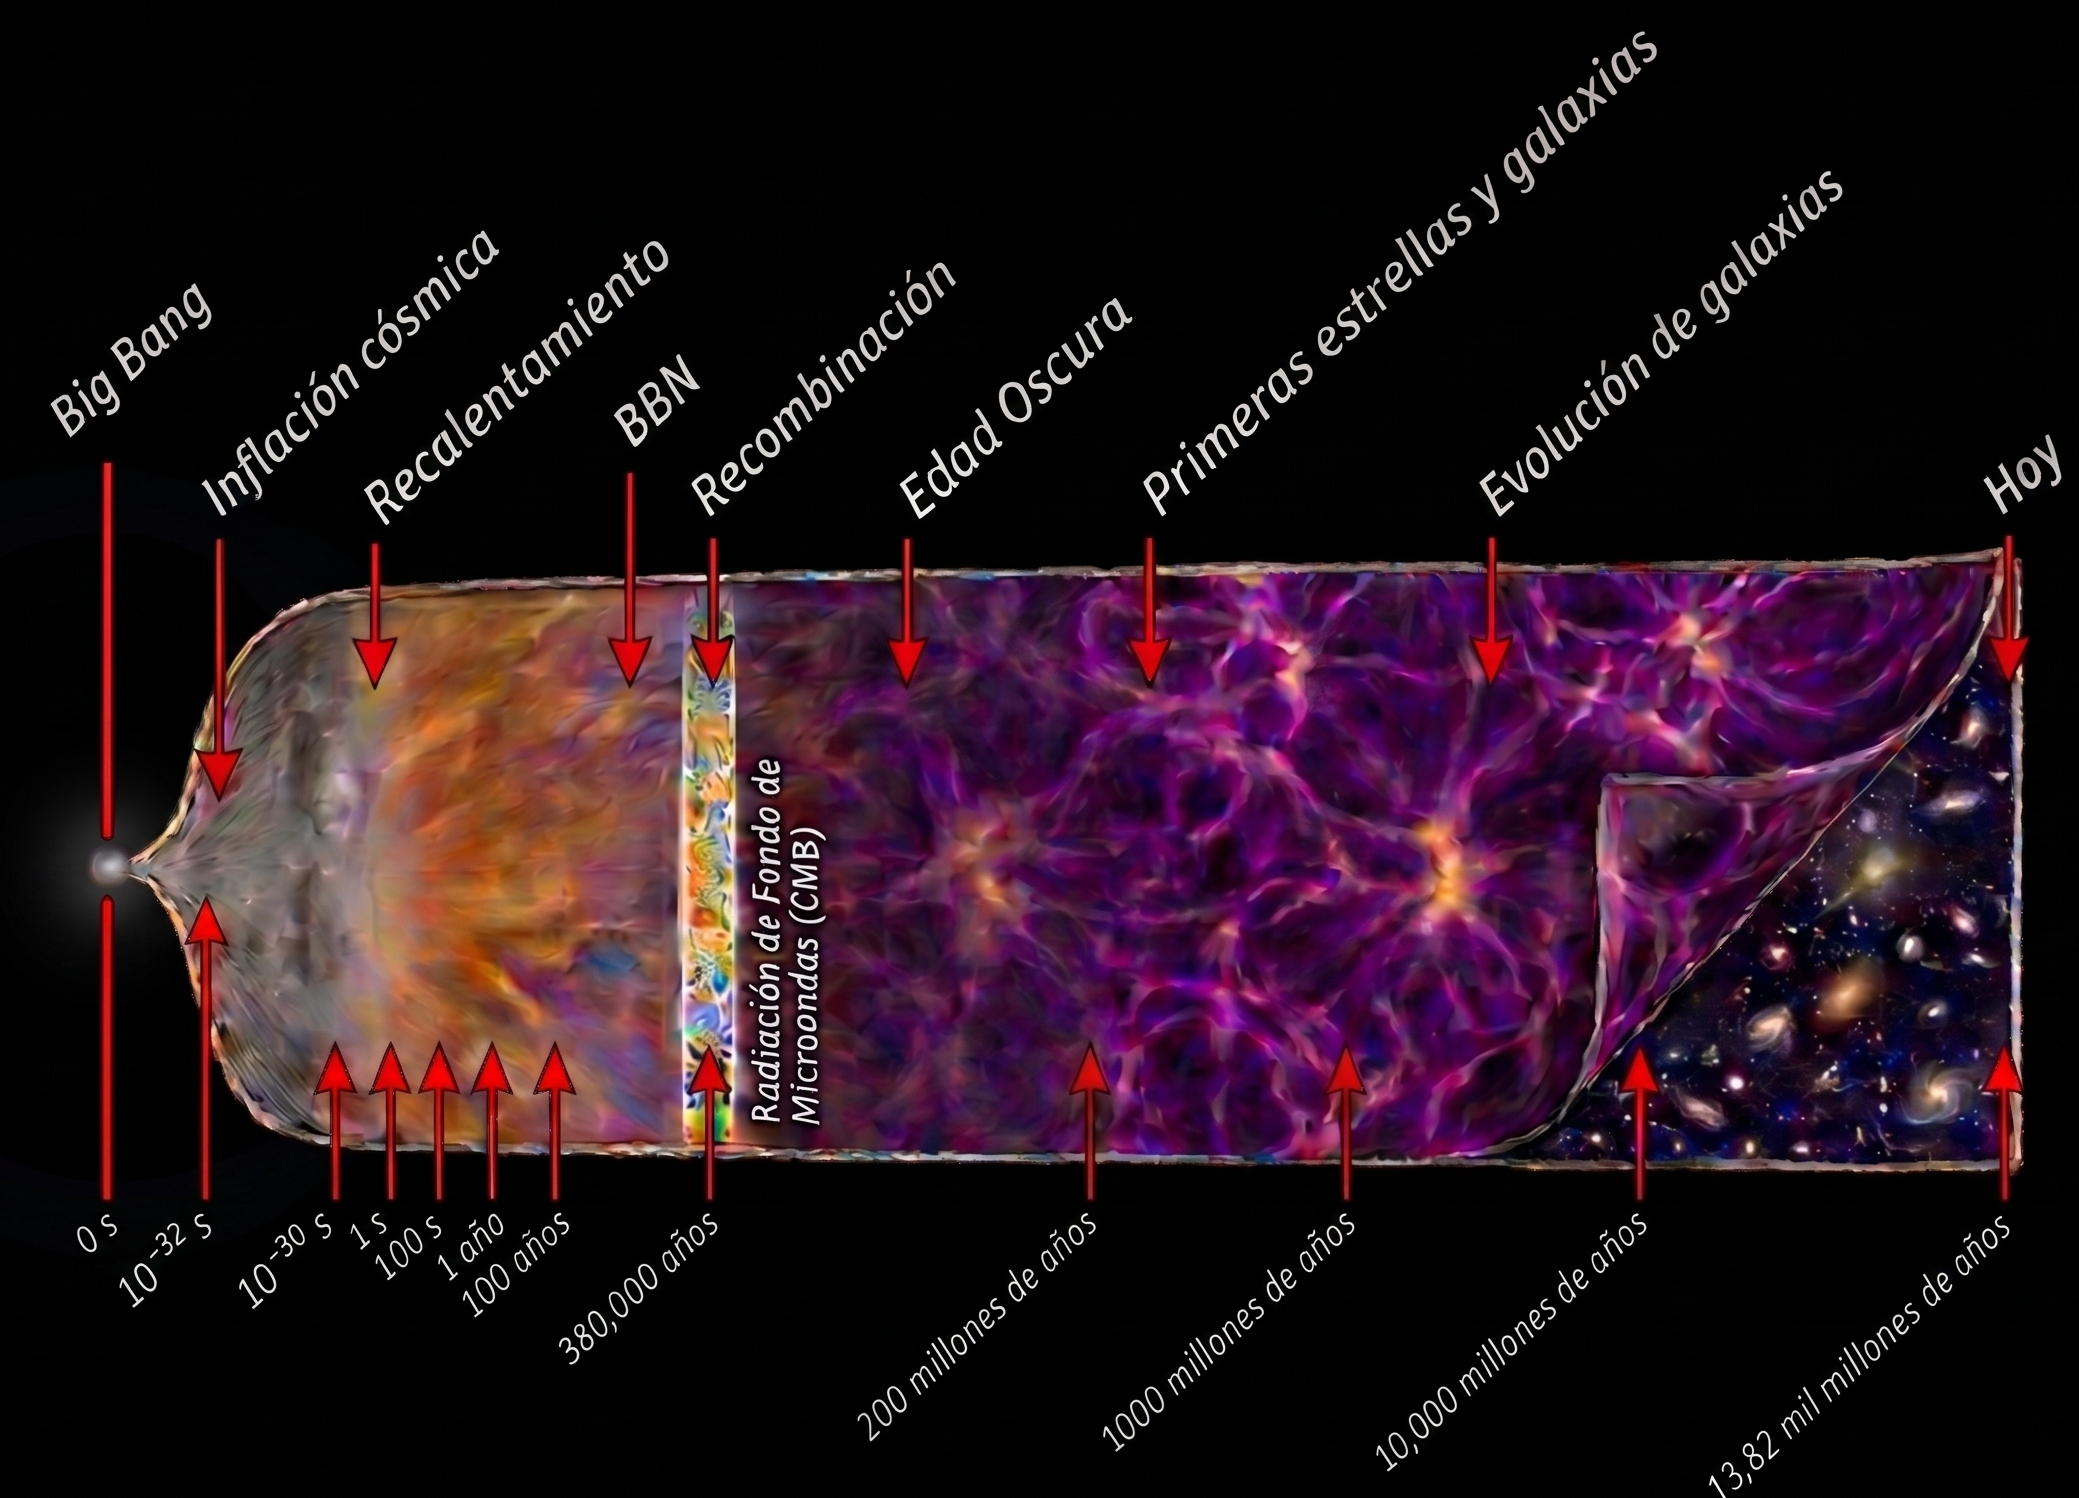
\includegraphics[width = 0.9\linewidth]{Figures/Cosmologia_etapas.png}};
                    \end{tikzpicture}
                \end{figure}
            \end{frame}

            \begin{frame}{FLRW + Ecuaciones de Friedmann}
                \small{
                \begin{itemize}
                    \item[\textcolor{brown}{$\bullet$}] La geometría del espacio-tiempo está descripta por 
                        \begin{equation*}
                            ds^2 = - dt^2 + a^2 (t) ~ \left[ \frac{dr^2}{1 - K r^2} + r^2 \left( d\theta^2 + \sin^2 \theta ~ d\varphi^2 \right) \right]
                        \end{equation*}

                    \item[\textcolor{brown}{$\bullet$}] La energía y materia se puede describir como un fluido ideal
                        \begin{equation*}
                            T_{\mu\nu} = (\rho + P) u_\mu u_\nu + P ~ g_{\mu\nu}
                        \end{equation*}
                        
                    \item[\textcolor{brown}{$\bullet$}] Las ecuaciones que describen la dinámica del universo seran
                        \begin{equation*}
                            \left( \frac{\dot{a}}{a} \right)^2 = \frac{8 \pi G}{3} \rho \hspace{2cm} \frac{\ddot{a}}{a} = - \frac{4 \pi G}{3} (\rho + 3 P)
                        \end{equation*}
                        \begin{equation*}
                            \dot{\rho} + 3 H (\rho + P) = 0
                        \end{equation*}
                        \vspace{-0.4cm}
                        \begin{itemize}
                            \item[\textcolor{cyan}{$\Longrightarrow$}] Se agrega una ecuación de estado: $P = \omega \rho$, siendo $\omega = 0$ para materia, $\omega = \frac{1}{3}$ para radiación y $\omega = -1$ para energía oscura.
                        \end{itemize}
                \end{itemize}
                }                
            \end{frame}

            \begin{frame}{Perturbaciones Cosmológicas y SVT}
                
            \end{frame}

            \begin{frame}{Inflación}
                \begin{figure}[H]
                    \centering
                    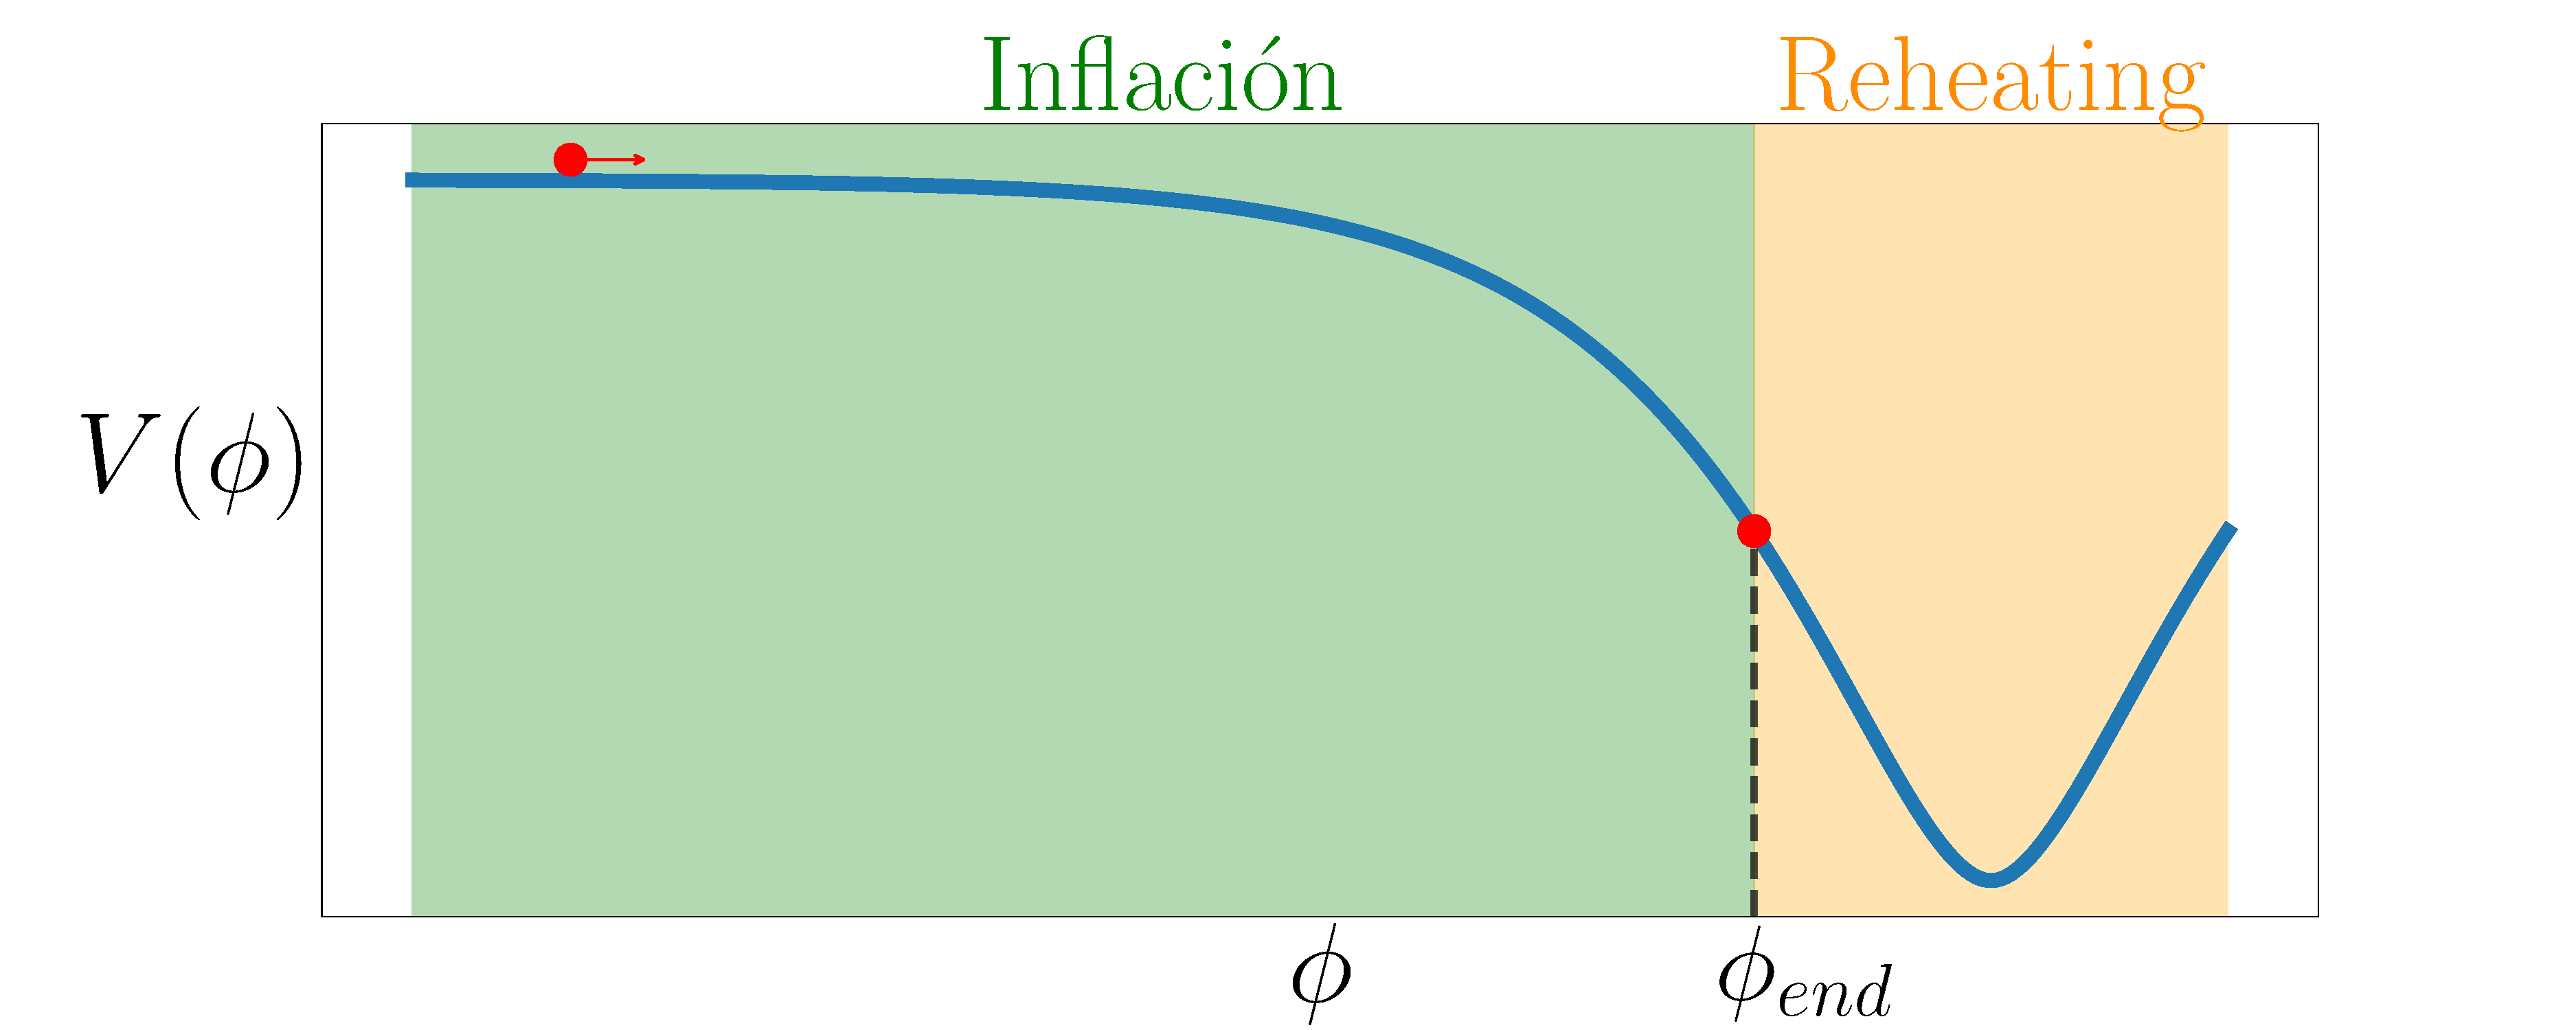
\includegraphics[width = \linewidth]{Figures/slow-roll.pdf}
                \end{figure}
            \end{frame}

            \begin{frame}{Recalentamiento}
                \begin{figure}[H]
                    \centering
                    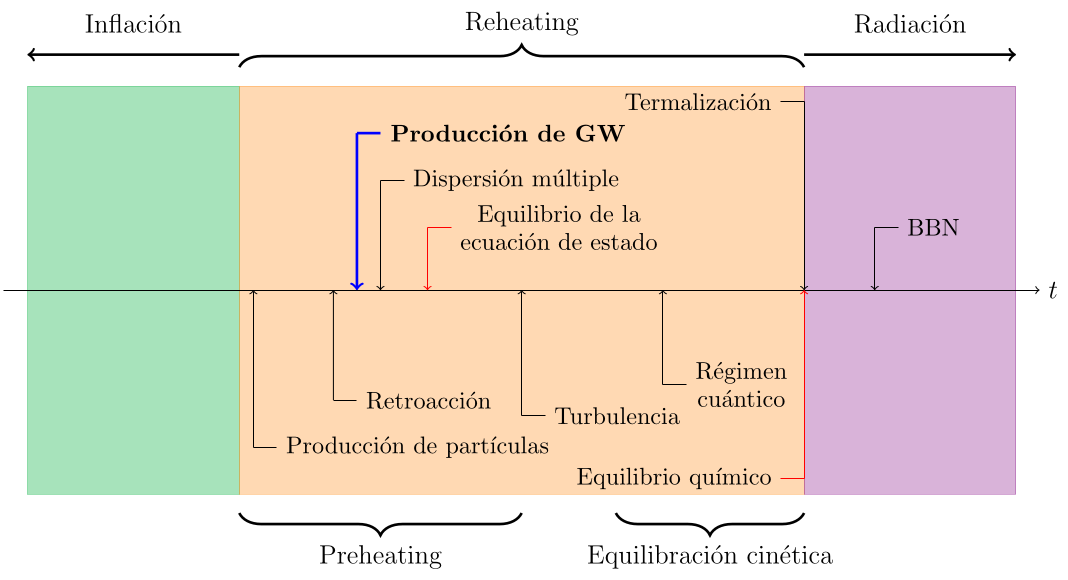
\includegraphics[width = \linewidth]{Figures/Reheating.png}
                \end{figure}
            \end{frame}

        \subsection{Ondas Gravitacionales}

            \begin{frame}{¿Que son las GWs?}

            \end{frame}

            \begin{frame}{Polarizaciones}
                \begin{figure}[H]
                    \centering
                    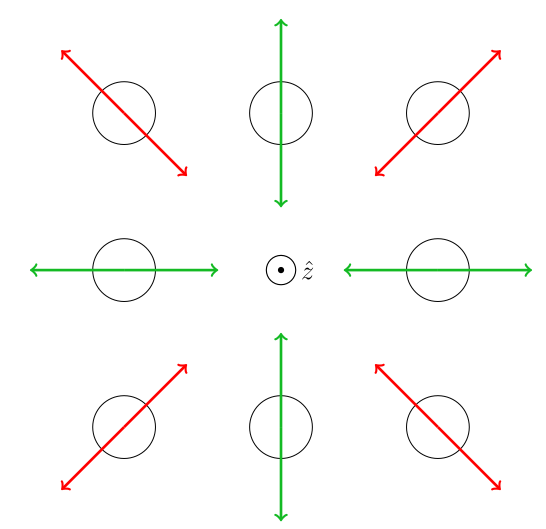
\includegraphics[width = 0.6\linewidth]{Figures/Polarizaciones_GWs.png}
                \end{figure}
            \end{frame}

            \begin{frame}{GWs en espacios curvos}
                
            \end{frame}

            \begin{frame}{Fondos estocásticos}
                
            \end{frame}

            \begin{frame}{Fuentes y detectores}
                \begin{figure}[H]
                    \centering
                    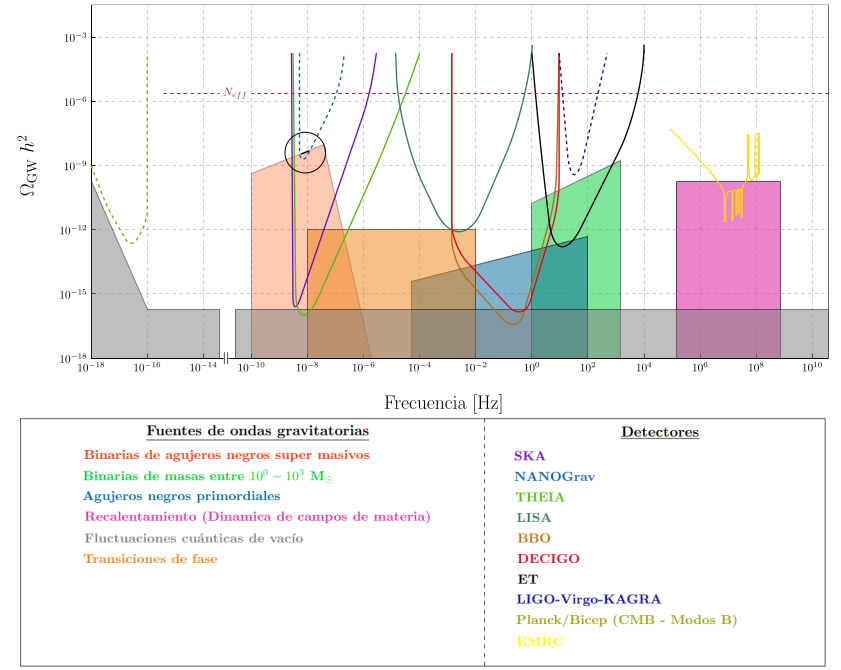
\includegraphics[width = 0.9\linewidth]{Figures/GW_detectors.png}
                \end{figure}
            \end{frame}

            \begin{frame}{Métodos de detección}
                \begin{figure}[H]
                    \centering
                    \begin{tikzpicture}
                        \node at (0,0) {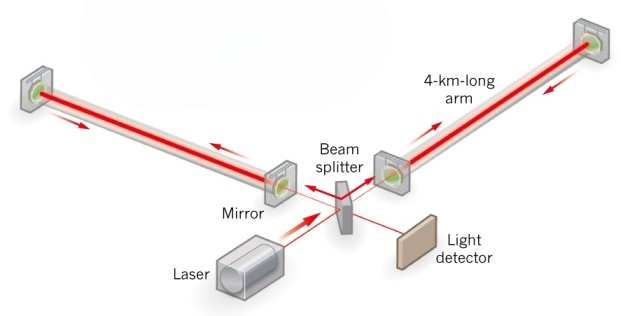
\includegraphics[scale = 0.4]{Figures/LIGO.jpg}};
                    \end{tikzpicture}
                \end{figure}                
            \end{frame}
            
    \begin{frame}
        \begin{figure}[H]
            \begin{tikzpicture}
                \node at (0,0) {\Huge \color{black}\contour{gold}{\uppercase{\textit{Preheating} Lineal}}};                
            \end{tikzpicture}
        \end{figure}
    \end{frame}

    \section{\textit{Preheating} lineal}

        \subsection{Resonancia Paramétrica}

            \begin{frame}{\textit{Preheating}}
            
            \end{frame}

            \begin{frame}{\textit{Background}}
                \begin{figure}[H]
                    \centering
                    \begin{subfigure}[t]{0.7\linewidth}
                        \centering
                        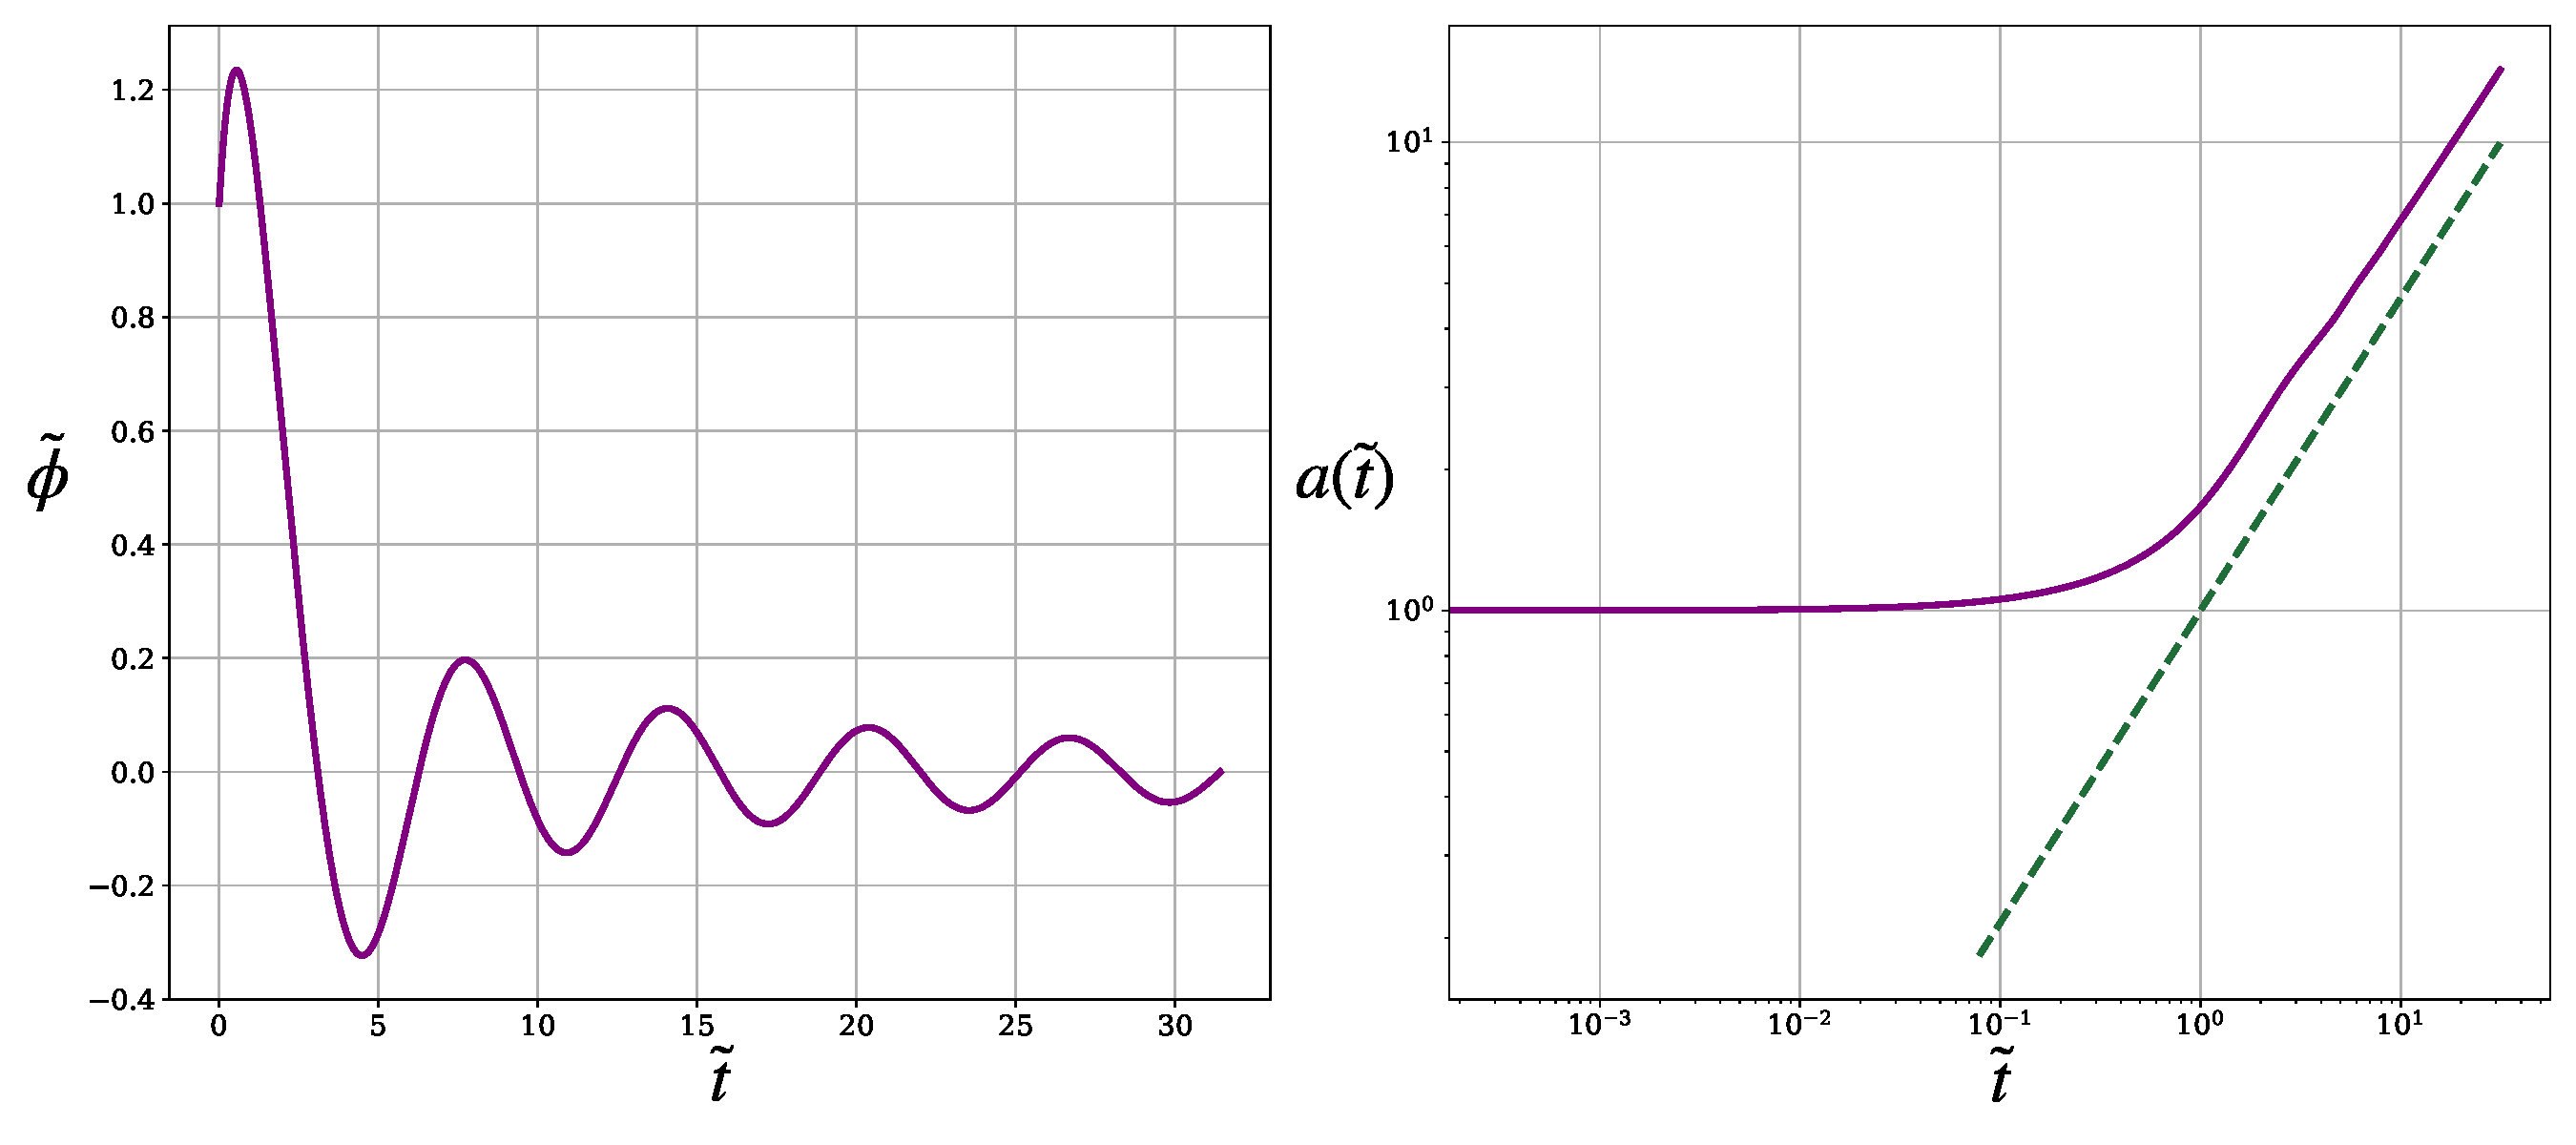
\includegraphics[width = \linewidth]{Figures/background_m2phi2.pdf}
                        \subcaption{$m^2 \phi^2$}
                    \end{subfigure}

                    \begin{subfigure}[b]{0.7\linewidth}
                        \centering
                        \includegraphics[width = \linewidth]{Figures/background_lphi4.pdf}
                        \subcaption{$\lambda \phi^4$}
                    \end{subfigure}
                \end{figure}
            \end{frame}

            \begin{frame}{Perturbaciones}
                
            \end{frame}

        \subsection{Dinámica de los campos sin expansión: análisis de Floquet}

            \begin{frame}{Análisis de Floquet}
                
            \end{frame}

            \begin{frame}{Tablas de inestabilidades}
                \begin{figure}[H]
                    \centering
                    \begin{tikzpicture}
                        \node at (0,0) {
\includegraphics[width = \linewidth]{Figures/Floquet_lphi4.pdf}};
                    \end{tikzpicture}
                \end{figure}
            \end{frame}

            \begin{frame}{Amplificación por bandas: analisis exponente de Floquet}
                \begin{figure}[H]
                    \centering
                    \begin{tikzpicture}
                        \node at (0,0) {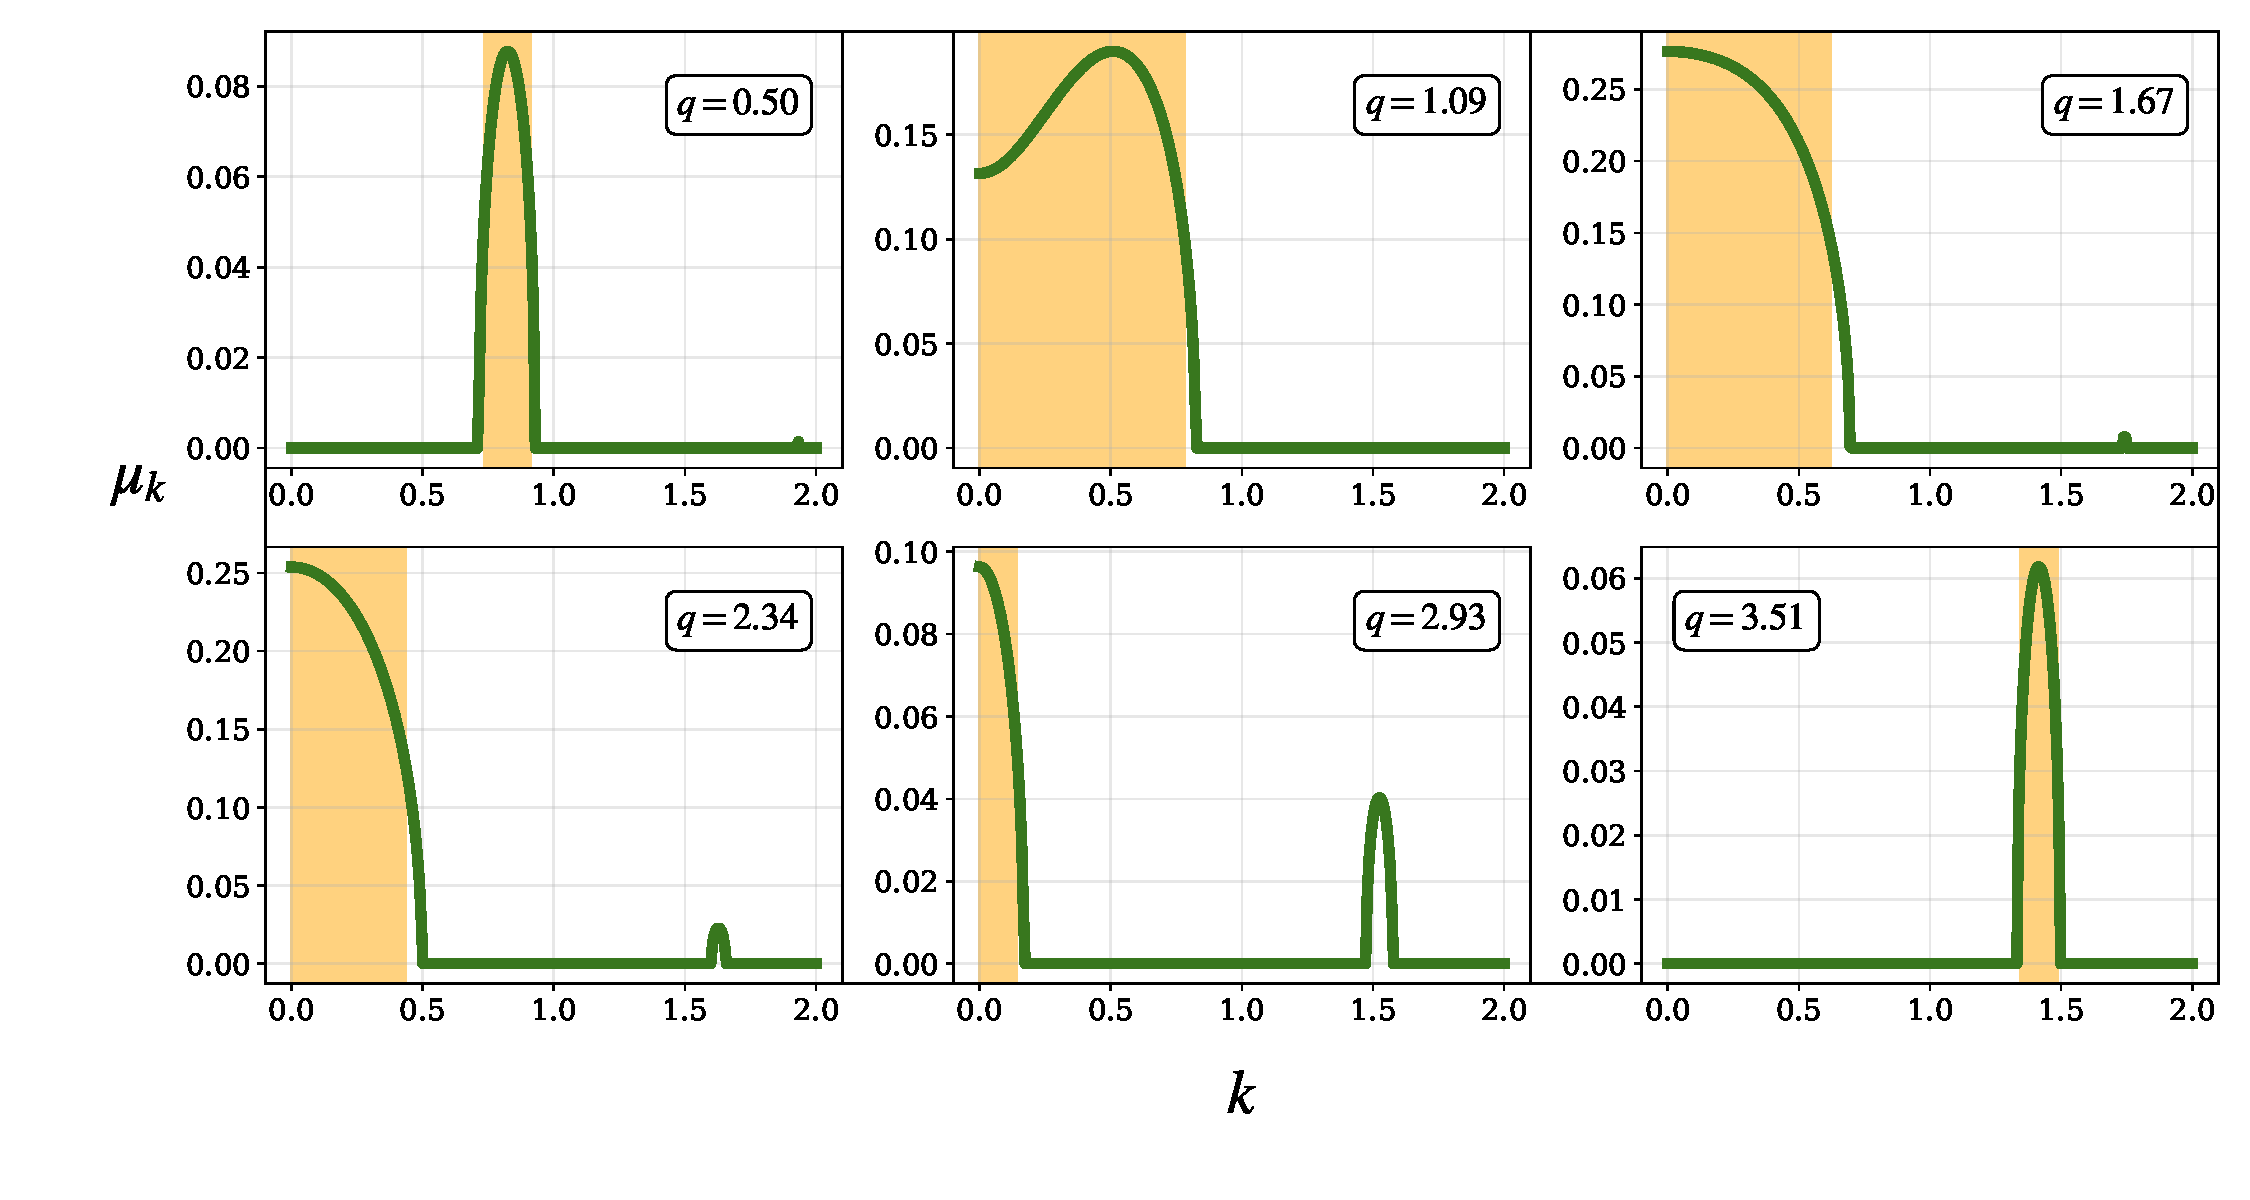
\includegraphics[width = 0.9\linewidth]{Figures/muk_lphi4.pdf}};
                    \end{tikzpicture}
                \end{figure}
            \end{frame}

            \begin{frame}{Tipos de resonancia: \textit{Narrow resonance}}
                \begin{figure}[H]
                    \centering
                    \begin{tikzpicture}
                        \node at (-3,2) {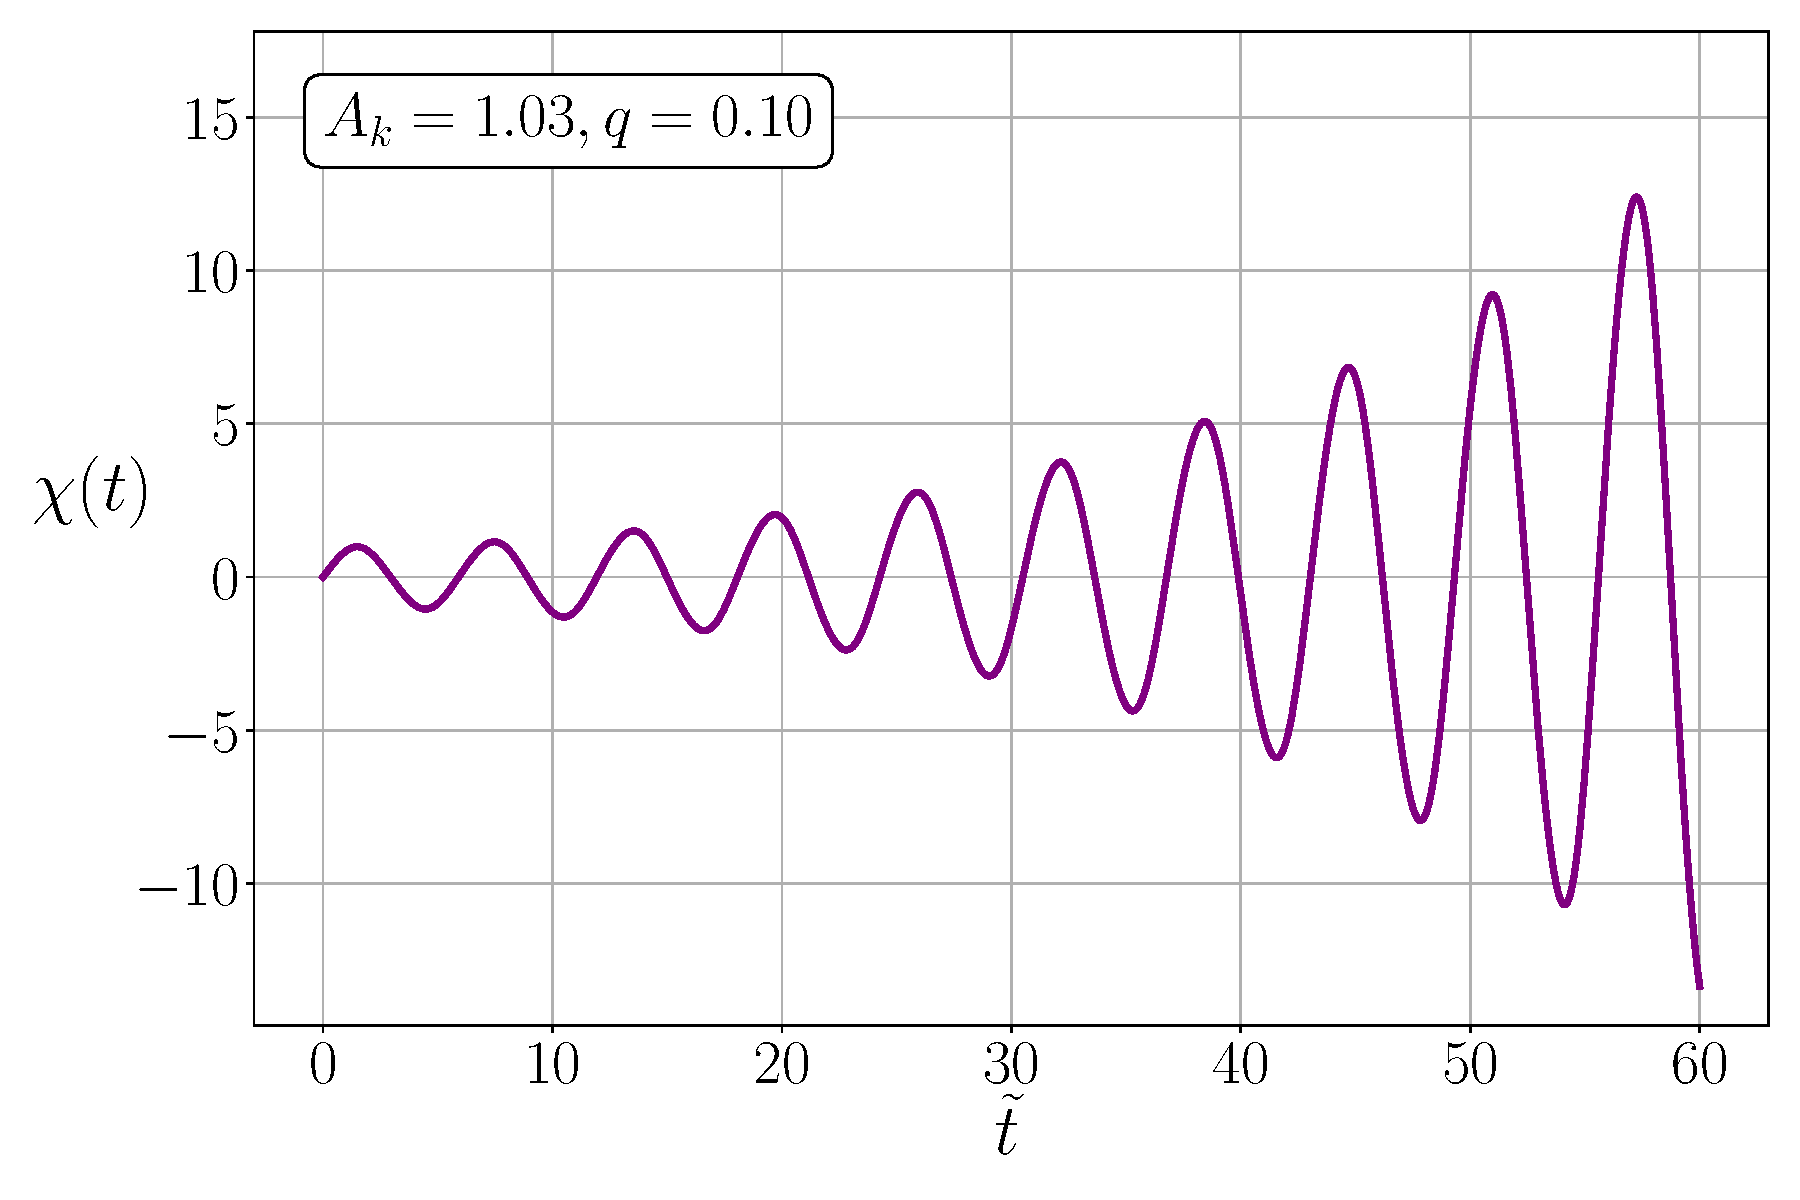
\includegraphics[width = 0.5\linewidth]{Figures/narrow_resonance_m2phi2.pdf}};
                        \node at (1.5,-2) {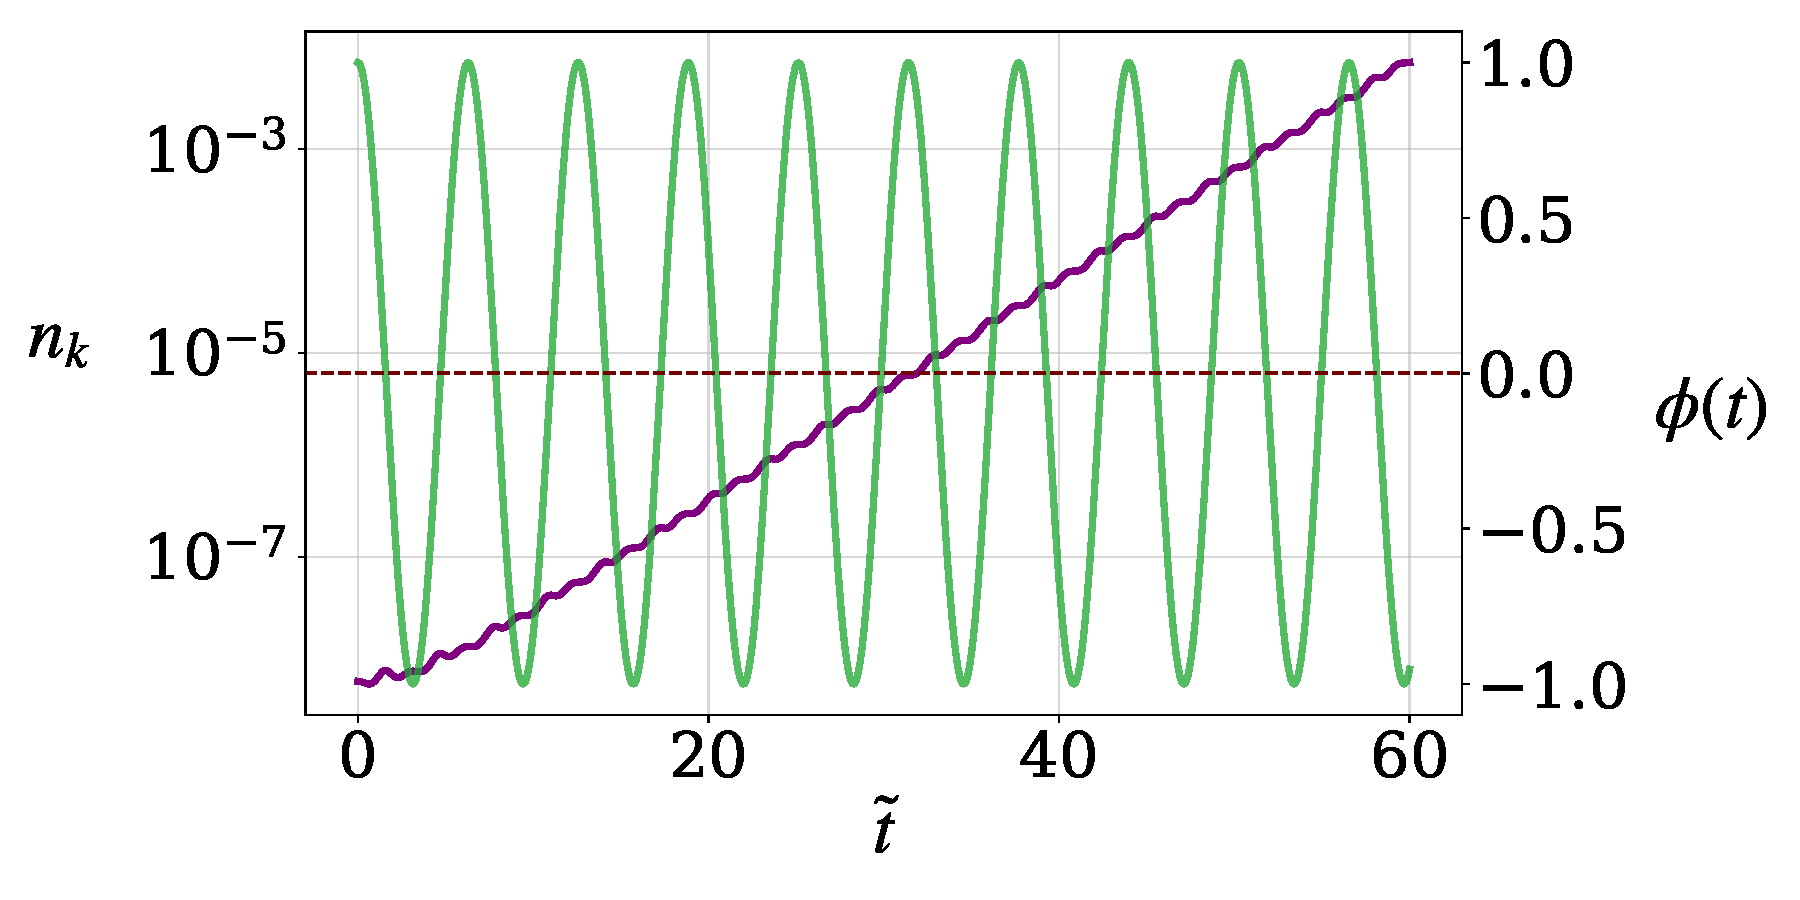
\includegraphics[width = 0.6\linewidth]{Figures/nk_Narrow_Resonance_m2phi2.pdf}};
                    \end{tikzpicture}
                \end{figure}
            \end{frame}

            \begin{frame}{Tipos de resonancia: \textit{Broad resonance}}
                \begin{figure}[H]
                    \centering
                    \begin{tikzpicture}
                        \node at (-3,2) {\includegraphics[width = 0.5\linewidth]{Figures/Broad_resonance_m2phi2.pdf}};
                        \node at (1.5,-2) {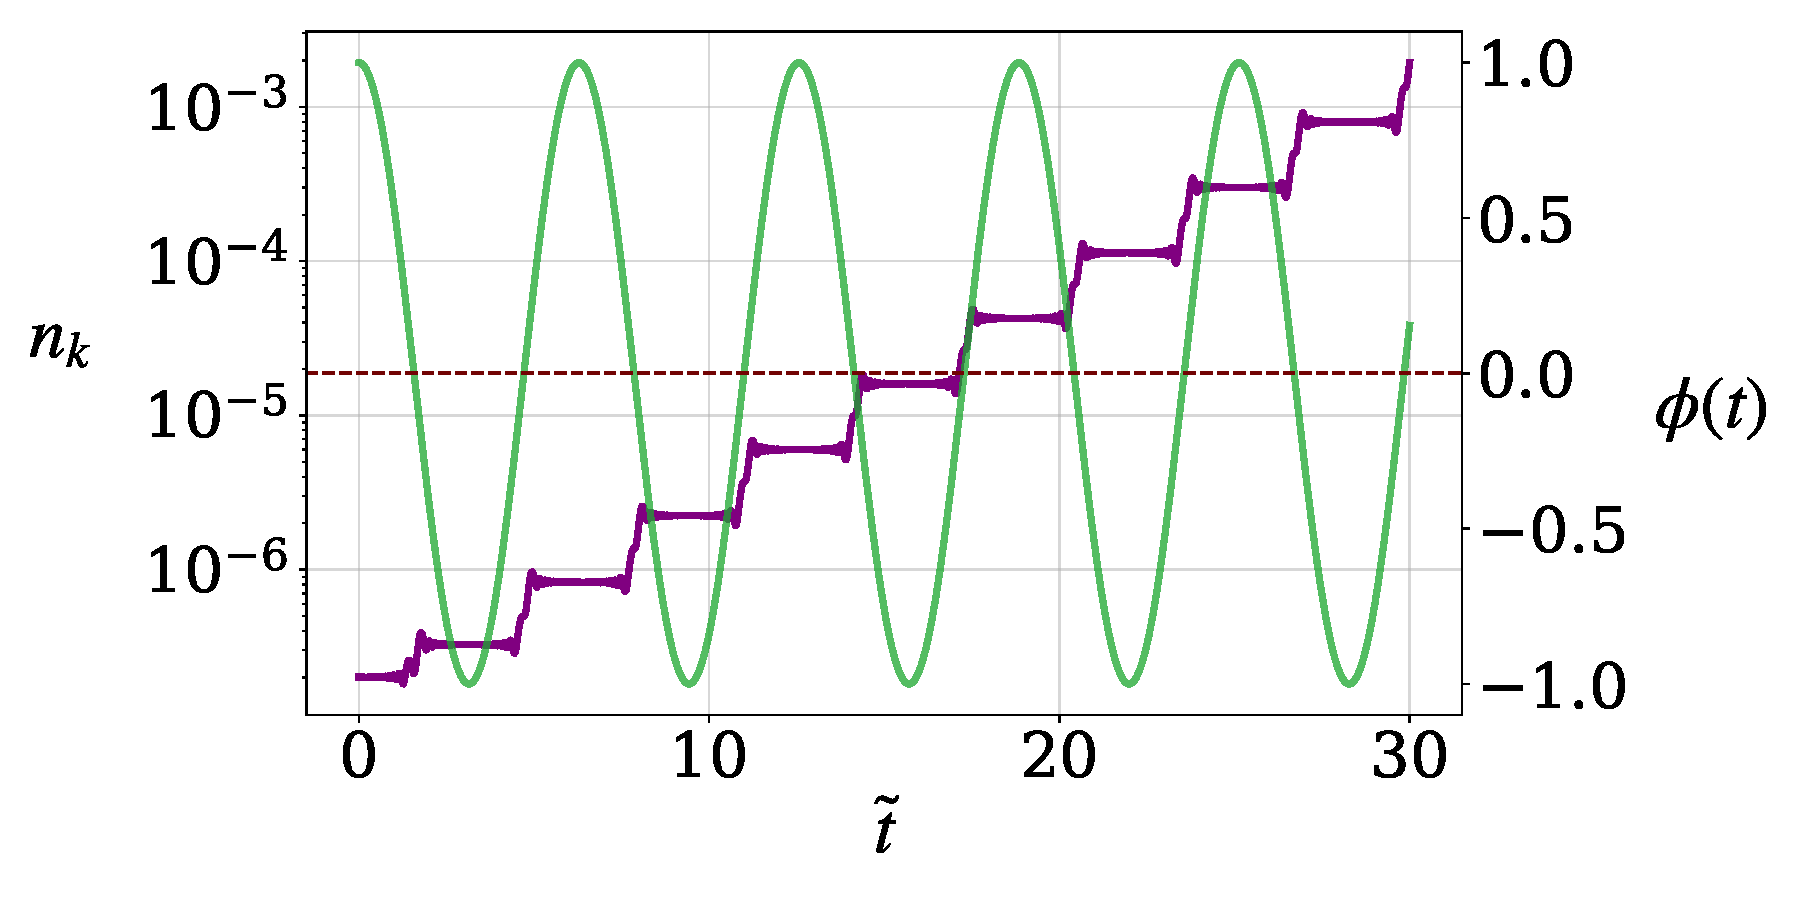
\includegraphics[width = 0.6\linewidth]{Figures/nk_Broad_Resonance_m2phi2.pdf}};
                    \end{tikzpicture}
                \end{figure}
            \end{frame}

        \subsection{Dinámica de los campos con expansión del universo}

            \begin{frame}{Caso $m^2 \phi^2$: \textit{Stochastic resonance}}
                \begin{figure}[H]
                    \centering
                    \begin{tikzpicture}
                        \node at (0,0) {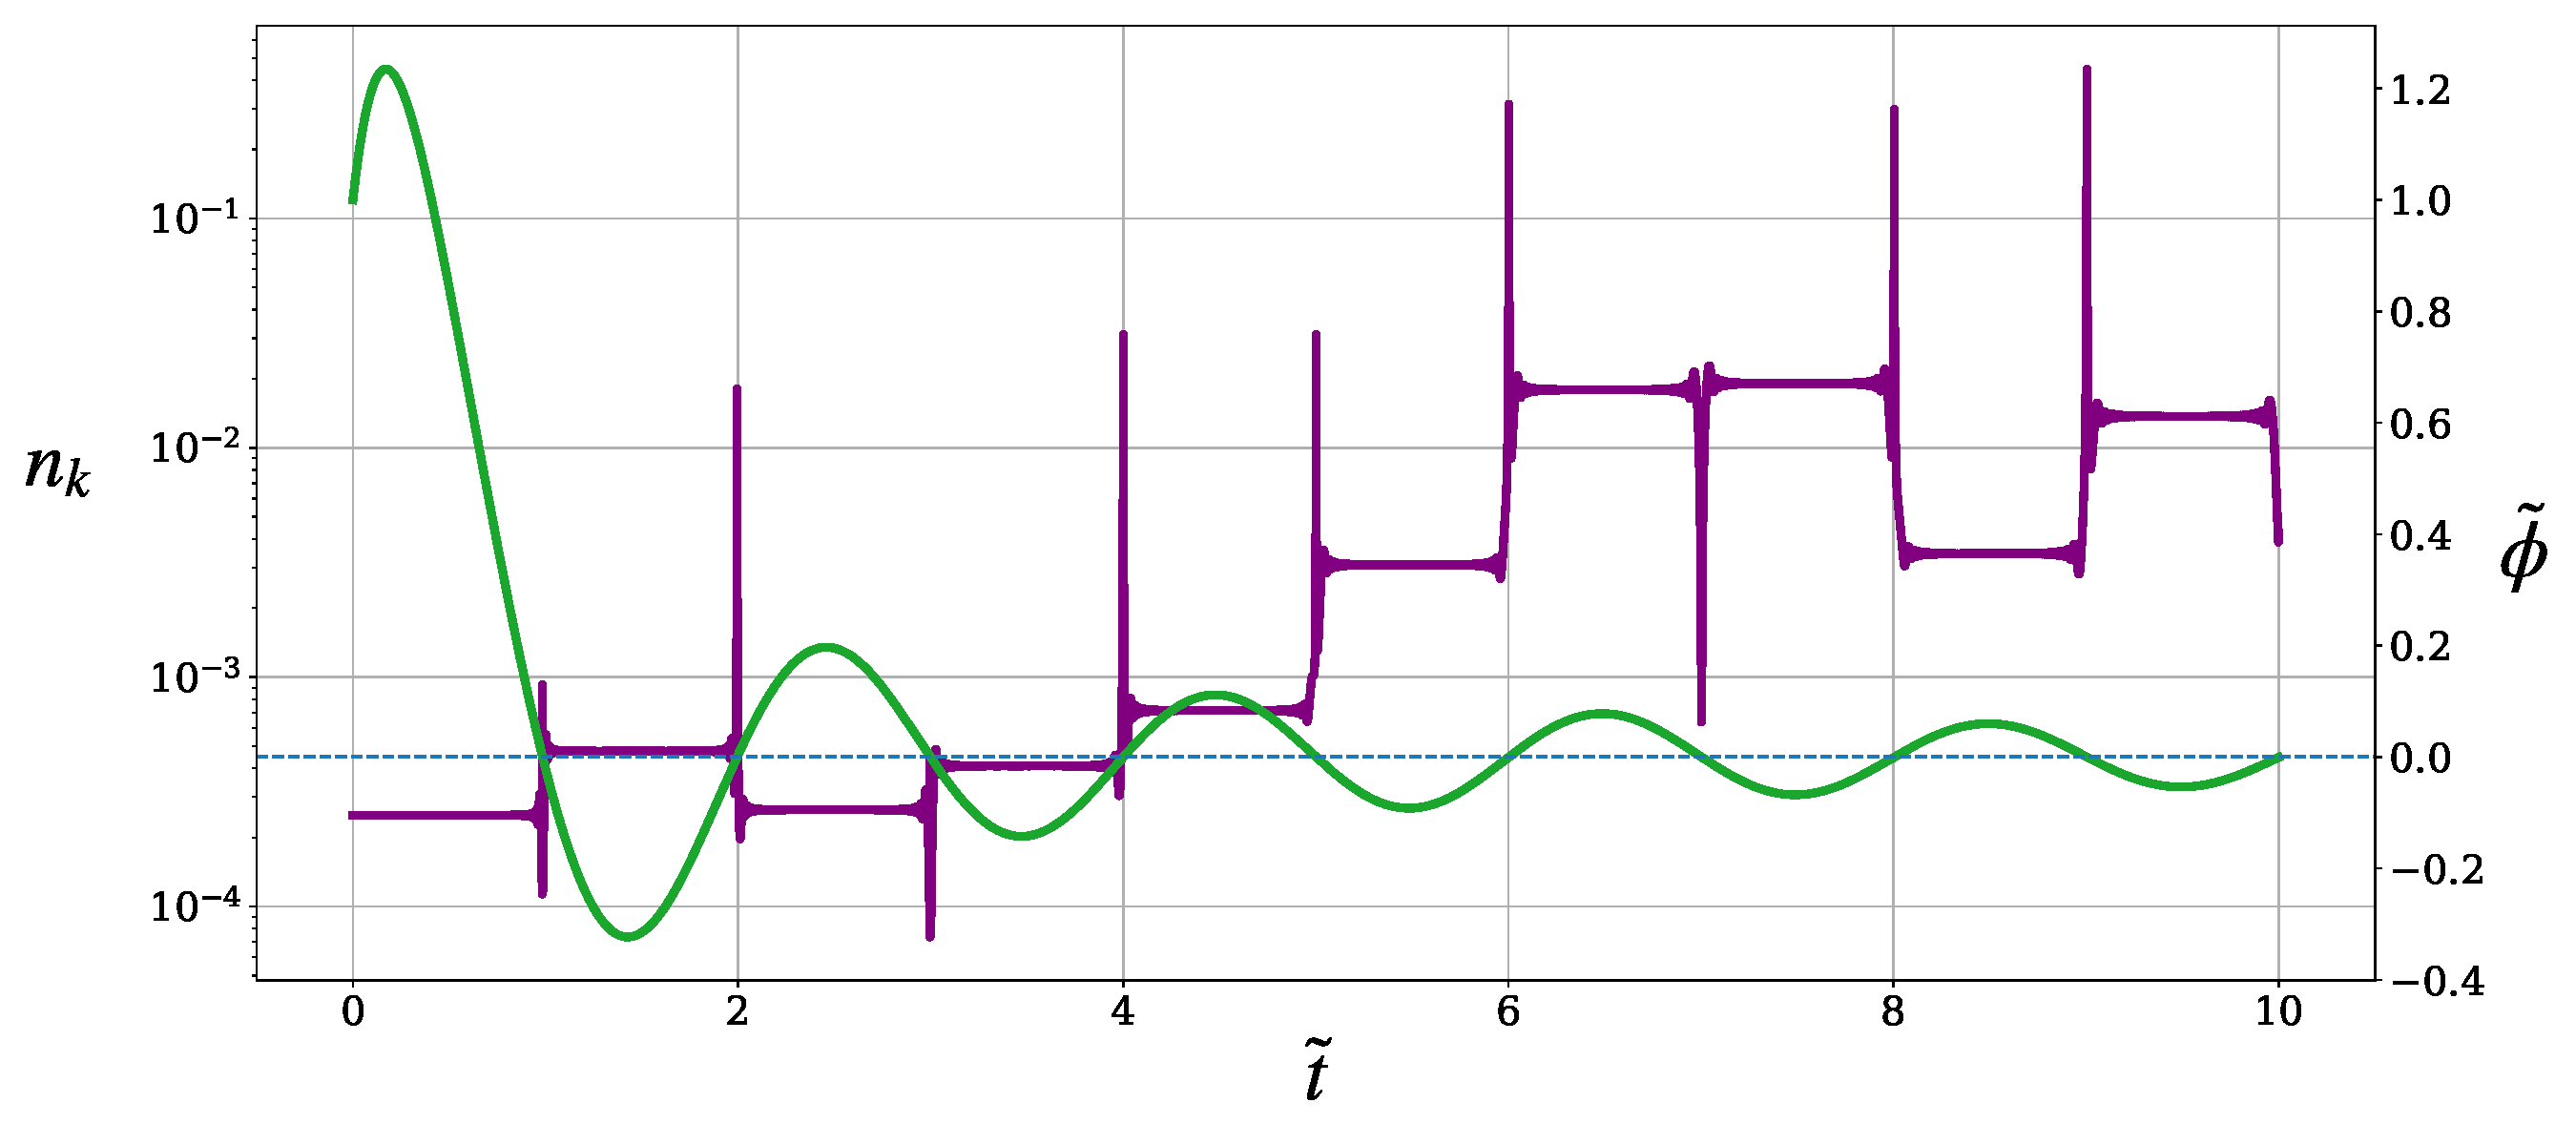
\includegraphics[width = 0.85\linewidth]{Figures/nk_Broad_resonance_expansion_m2phi2.pdf}};
                    \end{tikzpicture}
                \end{figure}
            \end{frame}

            \begin{frame}{Caso $\lambda \phi^4$}
            
            \end{frame}

        \subsection{Producción de ondas gravitacionales}

            \begin{frame}{Espectro de potencias de $\chi$}
                \begin{figure}[H]
                    \centering
                    \begin{tikzpicture}
                        \node at (0,0) {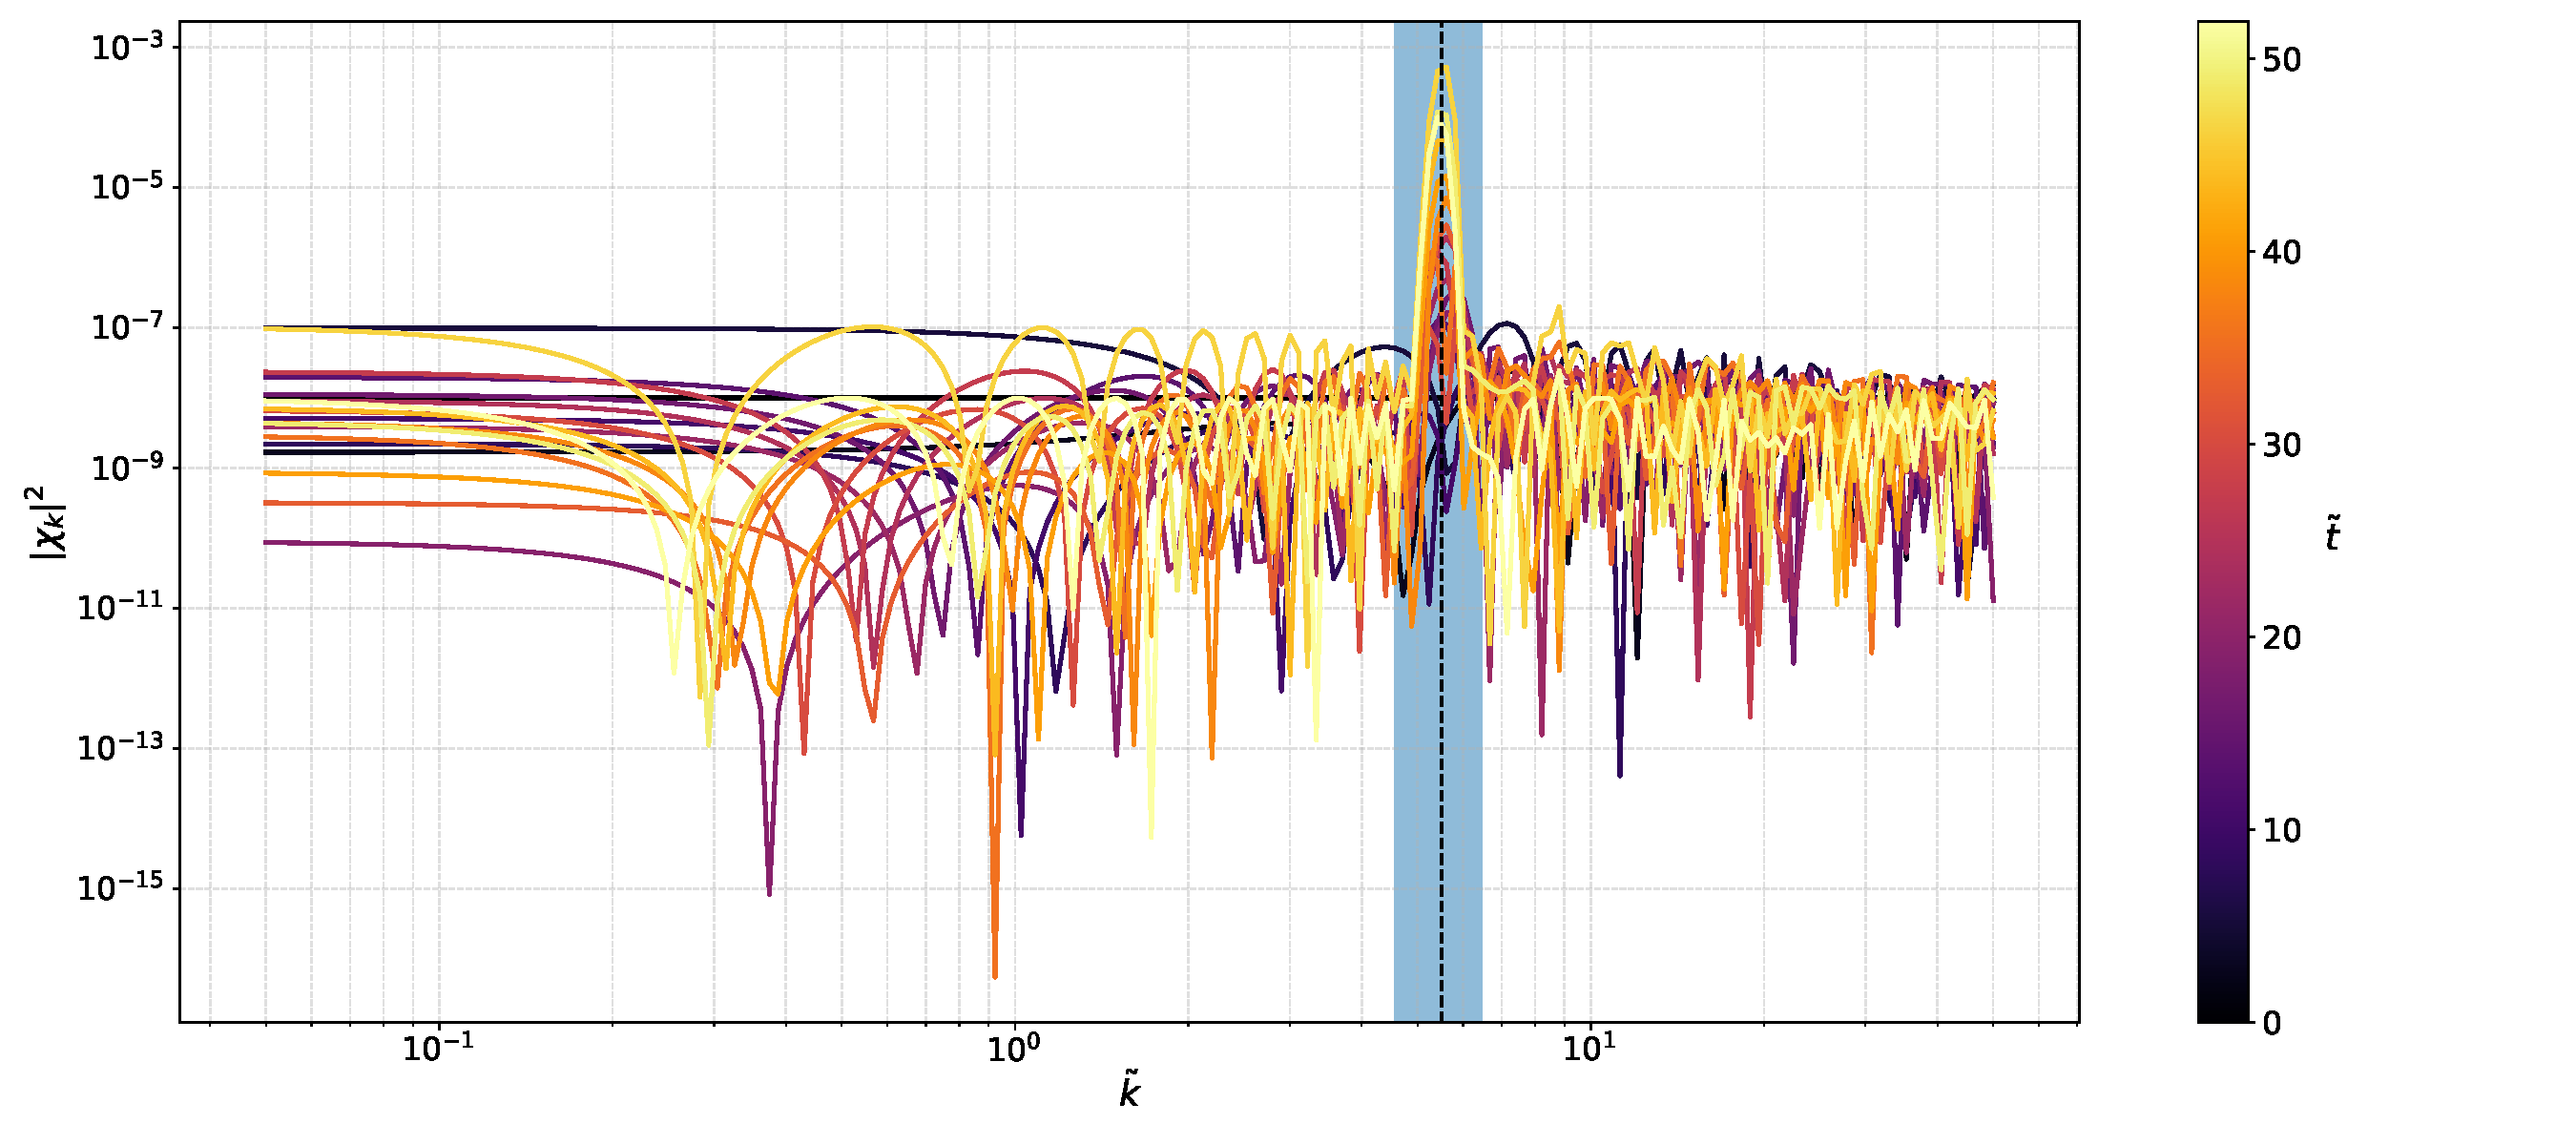
\includegraphics[width = 0.85\linewidth]{Figures/Pchi_lineal.pdf}};
                    \end{tikzpicture}
                \end{figure}
            \end{frame}

            \begin{frame}{Espectro de potencias para las ondas gravitacionales}
                \begin{figure}[H]
                    \centering
                    \begin{tikzpicture}
                        \node at (0,0) {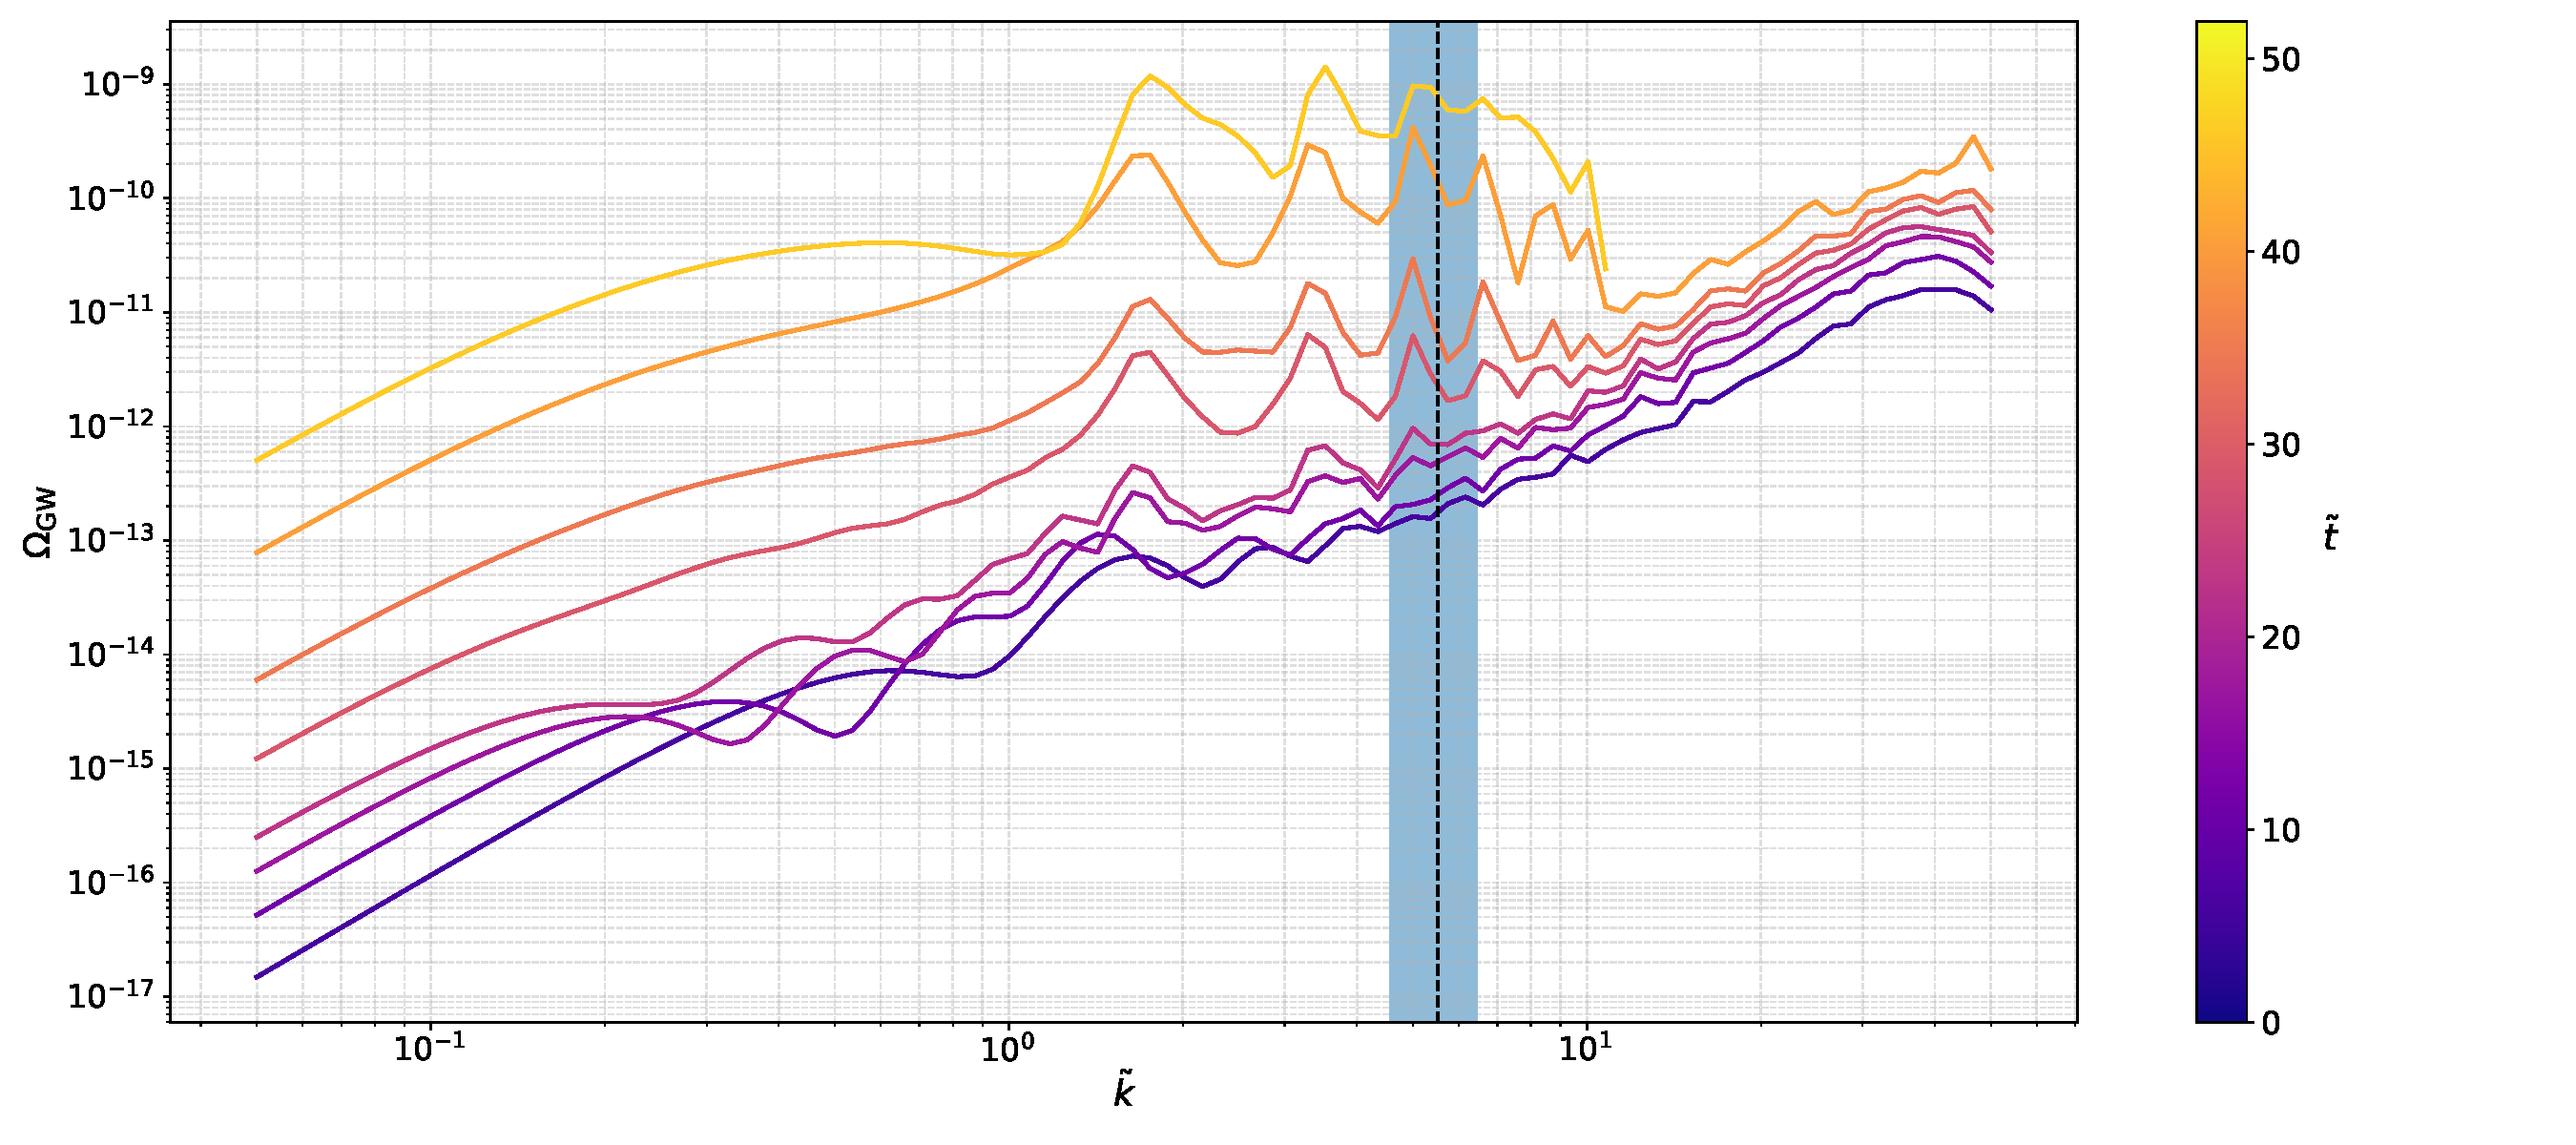
\includegraphics[width = 0.85\linewidth]{Figures/Omega_lineal.pdf}};
                    \end{tikzpicture}
                \end{figure}
            \end{frame}

    \begin{frame}
        \begin{figure}[H]
            \begin{tikzpicture}
                \node at (0,0) {\Huge \color{black}\contour{gold}{\uppercase{\CosmoLattice}}};                
            \end{tikzpicture}
        \end{figure}
    \end{frame}

    \section{\CosmoLattice}

        \subsection{¿Qué es?}

            \begin{frame}{¿Qué es?}
                \begin{figure}[H]
                    \centering
                    \begin{tikzpicture}
                        \node at (0,0) {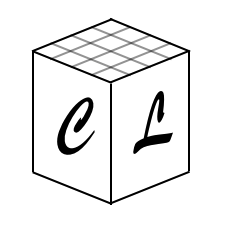
\includegraphics[scale = 0.4]{Figures/CL_Icon.png}};
                    \end{tikzpicture}
                \end{figure}
            \end{frame}

            \begin{frame}{Ecuaciones}
                
            \end{frame}

        \subsection{Comparación a tiempos cortos}

            \begin{frame}{Estudio de Floquet - tiempos cortos}
                \begin{figure}[H]
                    \centering
                    \begin{tikzpicture}
                        \node at (-2.25,2) {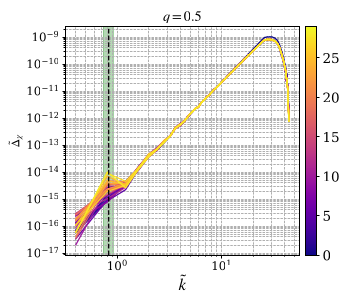
\includegraphics[width = 0.35\linewidth]{Figures/CL_Pchi_short1.png}};
                        \node at (2.25,2) {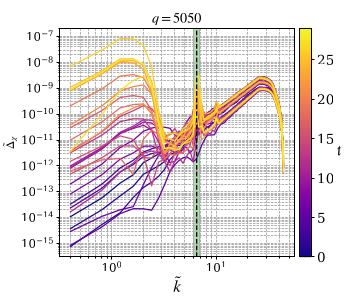
\includegraphics[width = 0.35\linewidth]{Figures/CL_Pchi_short2.png}};
                        \node at (-2.25,-2) {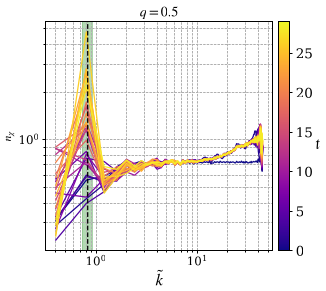
\includegraphics[width = 0.35\linewidth]{Figures/CL_nk_short1.png}};
                        \node at (2.25,-2) {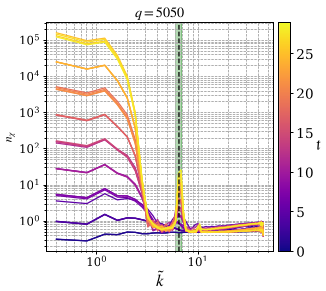
\includegraphics[width = 0.35\linewidth]{Figures/CL_nk_short2.png}};
                    \end{tikzpicture}
                \end{figure}
            \end{frame}

            \begin{frame}{Espectros de potencias para las ondas gravitacionales}
                \begin{figure}[H]
                    \centering
                    \begin{tikzpicture}
                        \node at (-2.5,0) {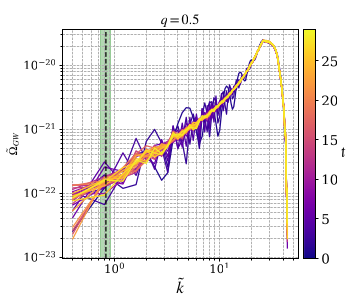
\includegraphics[width = 0.4\linewidth]{Figures/CL_Omega_short1.png}};
                        \node at (2.5,0) {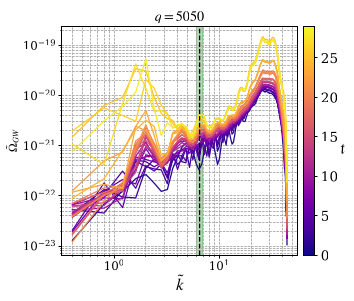
\includegraphics[width = 0.4\linewidth]{Figures/CL_Omega_short2.png}};
                    \end{tikzpicture}
                \end{figure}
            \end{frame}
        
        \subsection{Modelos de estudio}

            \begin{frame}{General}
                    
            \end{frame}

            \begin{frame}{Modelos de tipo radiación}
                \begin{figure}[H]
                    \centering
                    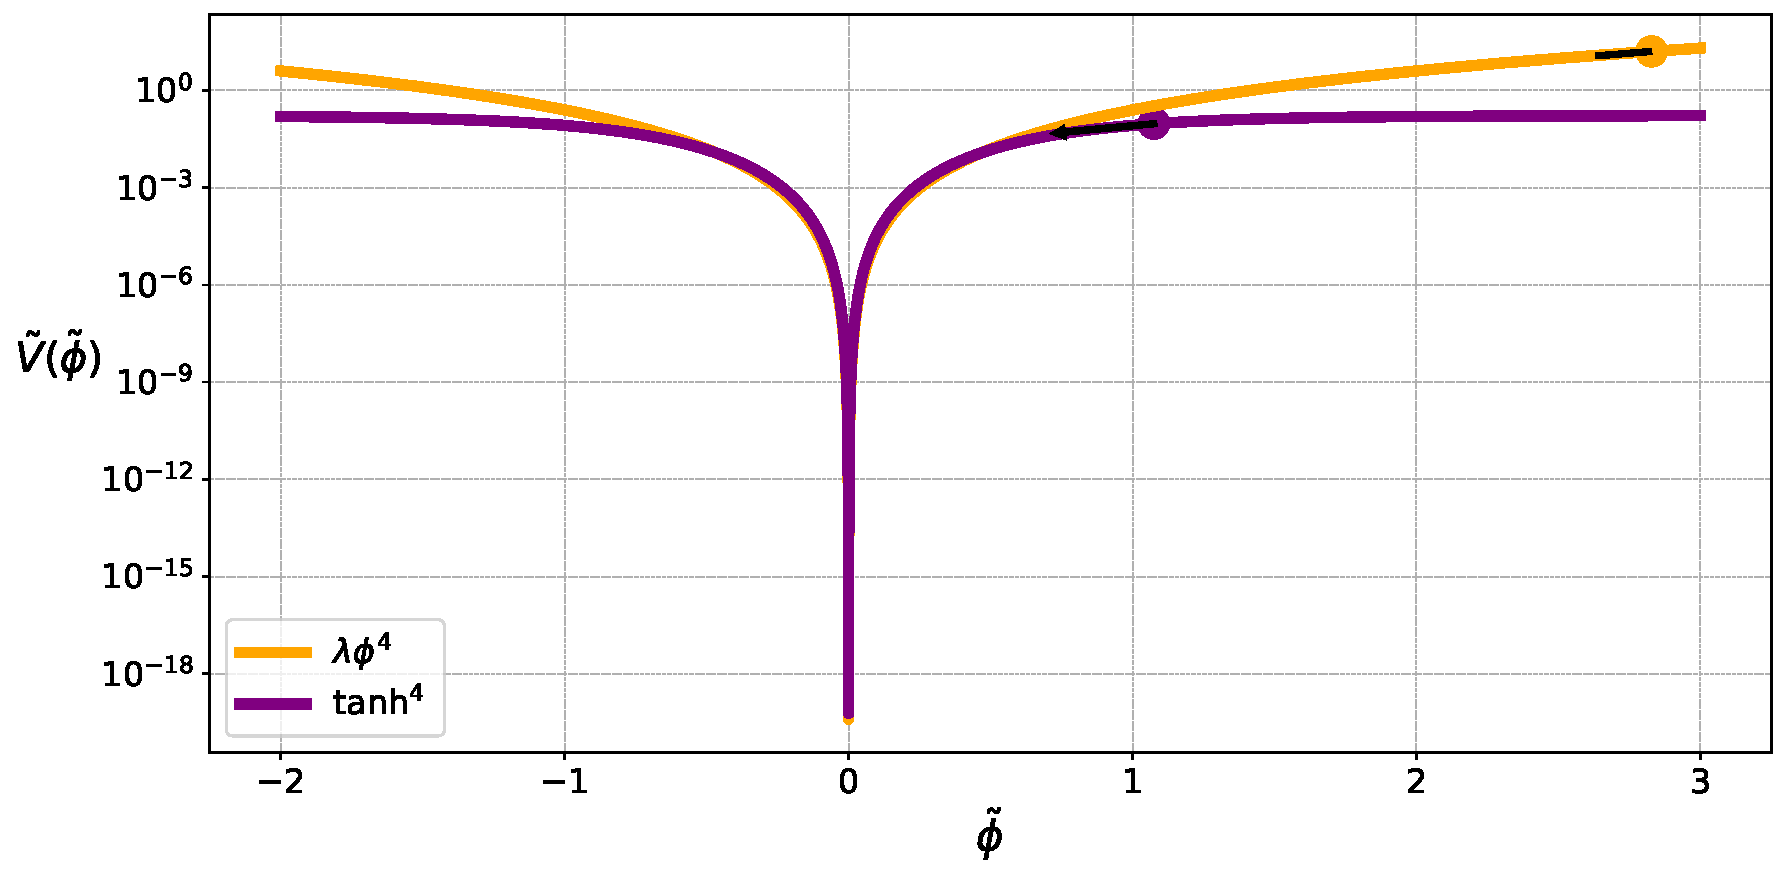
\includegraphics[width = 0.7\linewidth]{Figures/comparacion_w13.pdf}
                \end{figure}    
            \end{frame}

            \begin{frame}{Modelos de tipo materia}
                \begin{figure}[H]
                    \centering
                    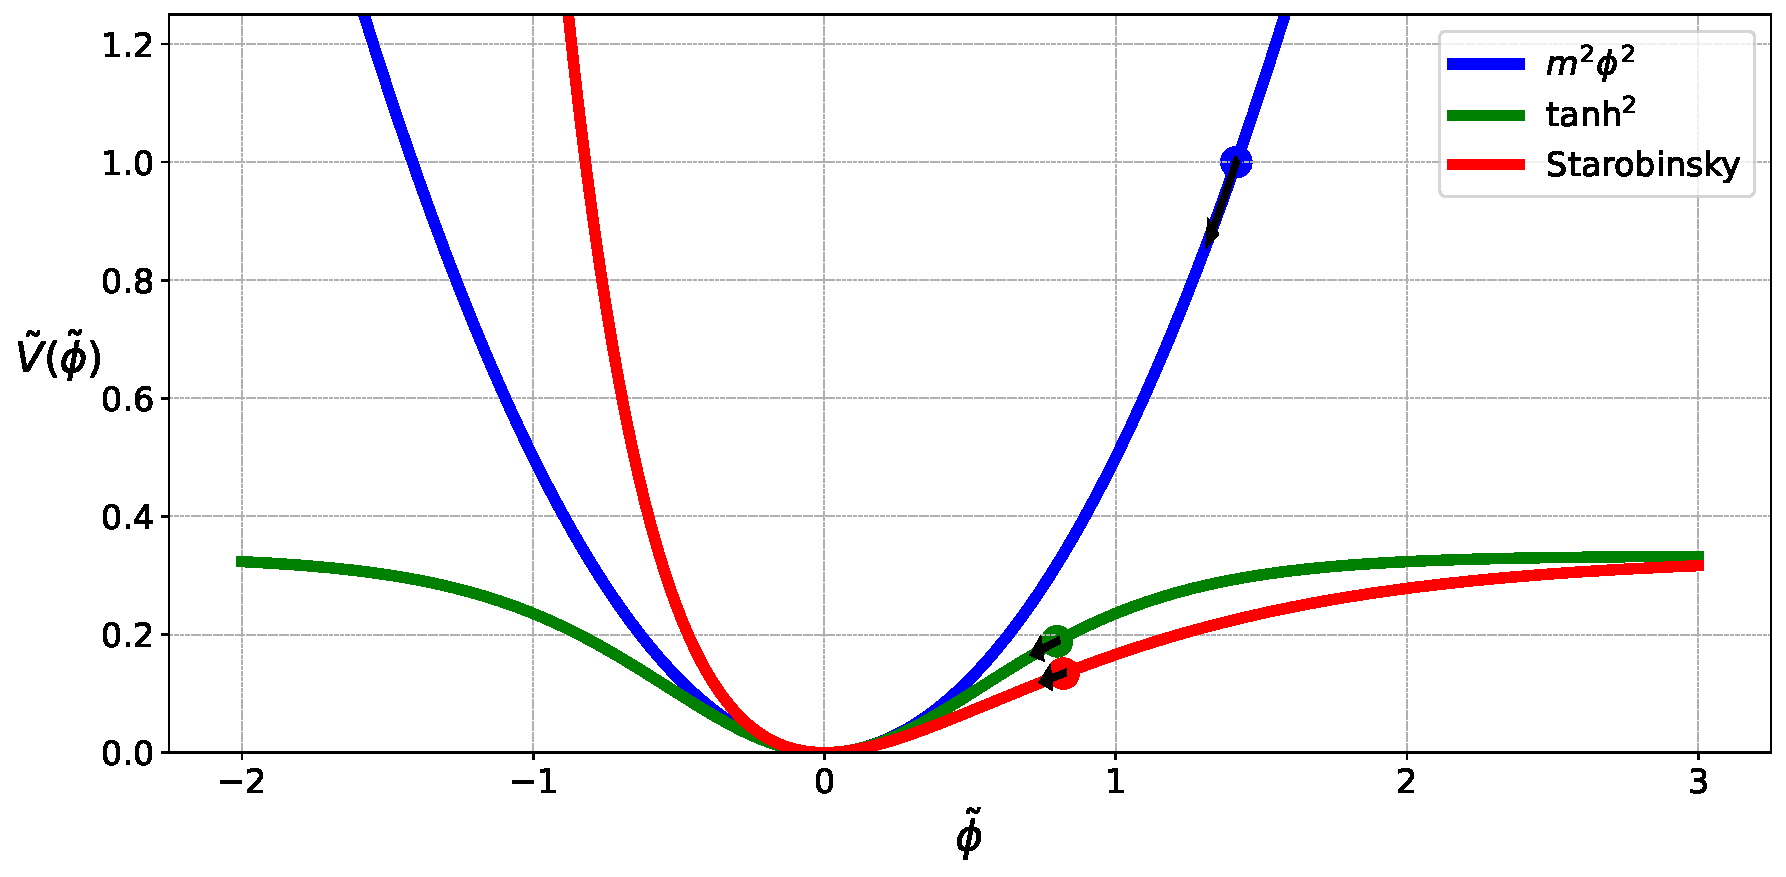
\includegraphics[width = 0.7\linewidth]{Figures/comparacion_w0.pdf}
                \end{figure}    
            \end{frame}

        \subsection{Comparación para modelos de tipo radiación}

            \begin{frame}{Comparación general 1}
                
            \end{frame}

            \begin{frame}{Comparación general 2}
                
            \end{frame}

            \begin{frame}{Barrido en los parámetros}
                
            \end{frame}

        \subsection{Comparación para modelos de tipo materia}

            \begin{frame}{Comparación general 1}
                
            \end{frame}

            \begin{frame}{Comparación general 2}
                
            \end{frame}

            \begin{frame}{Barrido en los parámetros}
                
            \end{frame}

        \subsection{Sensibilidad observacional y perspectivas de detección}

            \begin{frame}{Deformación característica}
                
            \end{frame}

            \begin{frame}{Perspectivas de detección}
                \begin{figure}[H]
                    \centering
                    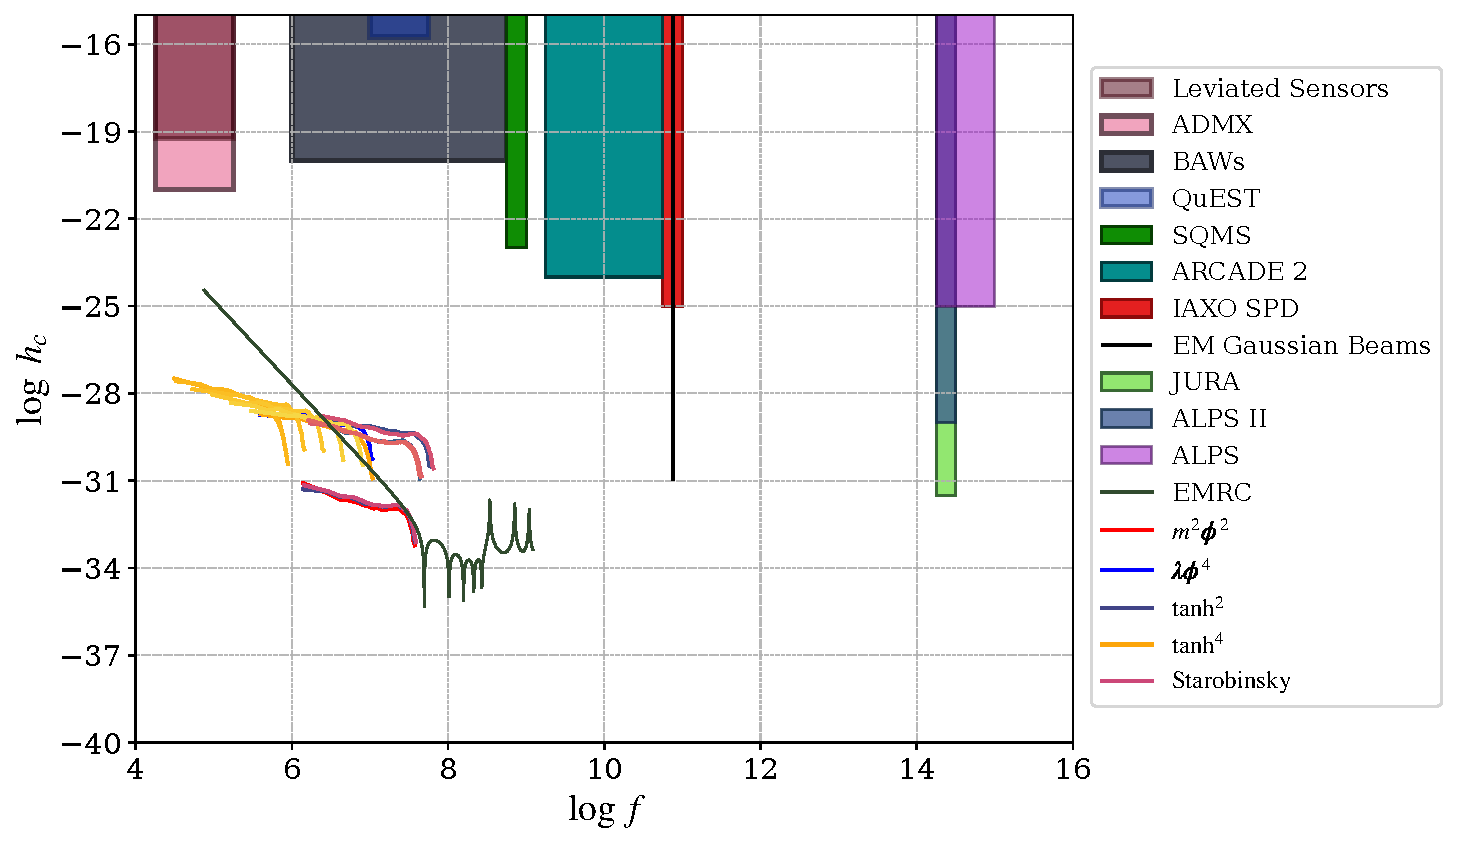
\includegraphics[width = 0.8\linewidth]{Figures/GW_Strain_Spectrum.pdf}
                \end{figure}
            \end{frame}

    \mostrarindicefalse % Apagamos el índice solo para la que viene

    \begin{frame}
        \begin{figure}[H]
            \begin{tikzpicture}
                \node at (0,0) {\Huge \color{black}\contour{gold}{\uppercase{Conclusiones}}};                
            \end{tikzpicture}
        \end{figure}
    \end{frame}

    \section{Conclusiones}

        \subsection{Conclusiones}

            \begin{frame}
                
            \end{frame}

        \subsection{Perspectivas a futuro}
        
            \begin{frame}
                
            \end{frame}

    \begin{frame}
        \begin{center}
            \Huge{Muchas Gracias}
        \end{center}
    \end{frame}

\end{document}